\def\year{2017}\relax \documentclass[letterpaper]{article}
\usepackage[left=2.5cm, right=2.5cm, top=2cm, bottom=2cm]{geometry}
\usepackage{authblk}
\usepackage{times}
\usepackage{helvet}
\usepackage{courier}
\usepackage{graphicx}
\usepackage{hyperref}
\usepackage{url}
\usepackage{graphicx}
\usepackage{amsmath}
\usepackage{amsfonts}
\usepackage{todonotes}
\usepackage{epstopdf}
\usepackage{color}
\usepackage{verbatim}
\usepackage{pdfpages}
\usepackage{ amssymb }
\usepackage{caption}
\usepackage{subcaption}
\usepackage{float}
 \usepackage{booktabs}
 \usepackage{colortbl}
 \usepackage{tabularx}

 \renewcommand{\arraystretch}{1.2}
\frenchspacing
\setlength{\pdfpagewidth}{8.5in}
\setlength{\pdfpageheight}{11in}

\title{Deep Learning Classification \\of Cheatgrass Invasion using \\Biophysical and Remote Sensing Data}
%\title{Vegetation Coverage Estimates using Deep \\Representations of
%          Ecological Niche Factors\\ and Multispectral Satellite Imagery}
%A deep learning [approach | method] to combining biophysical and [multi-sensor | remote sensing] data to map cheatgrass invasion
%
%A deep learning approach to mapping [an invasive plant | cheatgrass invasion] using biophysical and remote sensing data
%
%Deep learning classification of [an invasive plant | cheatgrass invasion] using biophysical and remote sensing data
% 

\author[1]{Kyle Larson\thanks{kyle.larson@pnnl.gov}}
\author[1]{Aaron Tuor\thanks{aaron.tuor@pnnl.gov}}
\affil[1]{Pacific Northwest National Laboratory}

%\setcounter{secnumdepth}{0}
\begin{document}
    \maketitle
	\tableofcontents

\begin{abstract} 
In this study we explore deep learning approaches which incorporate geophysical data and readings from multiple remote sensing platforms  for predictive mapping of vegetation over very large, ecologically diverse regions. We focus specifically on mapping an invasive exotic annual grass, cheatgrass ({\em Bromus tectorum}), that has become a major land management issue in the Western United States. We explore the relative advantages of deep neural networks to integrate imagery from the LandSat7 and MODIS platforms which have complementary advantages in their spectral bandwidth, spatial resolution, and temporal frequency. We show that integrating imagery from multiple platforms is beneficial to the predictive mapping of cheatgrass in the Western United State's historic range of Sage Grouse.  Our analysis of prospective machine learning models demonstrates that a deep neural network can more effectively take advantage of the signal from multiple platforms than traditional classification models such as Random Forest, and Linear Discriminant Analysis for the classification of cheatgrass.  
 \end{abstract}

%============================================================================================
%============================================================================================
%Section: Introduction================================================
%=============================================================================================
%============================================================================================
 \section{Introduction}
Accurate and up to date maps of vegetation coverage are critical assets for land management agencies tasked with mitigating damage wrought by invasive species. A variety of methods have been developed to map invasive annual grasses from satellite and aerial imagery, each uniquely tailored to the limitations of the imagery. Current practices usually involve choosing one platform best suited for the study, although more than one may potentially be useful, e.g.,  using finer spatial resolution imagery may improve
results, but doing so comes with concomitant loss of temporal resolution which is also important for
detecting species like invasive cheatgrass which has maintained a growth cycle distinct from native vegetation.


 Introduced in the late 19th-century, cheatgrass is now found in every state in the contiguous U.S.. Nowhere has its invasion been more prevalent than in western states where it has become a dominant component in many shrubland and grassland ecosystems. It is now estimated to dominate at least 40,000 km$^2$ in the states of Nevada and Utah alone. Cheatgrass invasion poses a variety of threats to ecosystem function, rangeland health, and human safety. A central thread to many of these threats is the increase in fine fuels associated with cheatgrass, which can lead to increased fire frequency and irreversible loss of native vegetation and wildlife habitat. Following a fire, cheatgrass is able to more effectively compete with native vegetation, giving rise to a positive feedback cycle of further invasion and fire.\texttt{ [Refs: Mack 1981; Pellant 1996; Bradley \& Mustard 2005; USDA Plant Database]}

While cheatgrass is considered ubiquitous throughout much of the western U.S., detailed spatial information about its presence and abundance are still lacking for much of its range within this region. Previous efforts to map cheatgrass have focused on core areas of invasion such as the Great Basin and Snake River Plain. These efforts help paint a clearer picture of cheatgrass invasion in the western U.S., but their disparate nature (due to differing extents, methods, data, and focal periods) prevents easily reconciling them to inform range-wide management decisions. Conversely, mapping cheatgrass (or other vegetation) at a range-wide scale is also not straightforward or without its challenges; most notably the need for a greater volume of training and input predictor data to adequately model the phenomenon across many ecological gradients. [Refs: ]

 
The study area encompasses a large part of the Intermountain West as well as portions of Montana, Wyoming, Colorado, and New Mexico east of the Rockies.  The areal extent of the area identified as the historic sage-grouse range covers more than 308 million acres and includes portions of southern Alberta and British Columbia, Canada.  This study focused on the U.S. portion of the sage-grouse range, which is approximately 288 million acres.
Figure \ref{fig:studyarea} shows the region considered and location of field samples.

%============================================================================================
%============================================================================================
%Section: Related Work================================================
%=============================================================================================
%============================================================================================
\section{Related Work}
\subsection{Cheatgrass Mapping}
A variety of methods to map cheatgrass are described in the literature, ranging from imagery-driven methods that focus on spectral signatures or phenological indicators of cheatgrass to ecological niche modeling approaches aimed at mapping biophysical and climatic predictors. Much attention has been given to deriving phenological indicators of cheatgrass presence from overhead imagery (typically using spectral indices such as the Normalized Difference Vegetation Index, or NDVI) because its life cycle differs from many of the native plant species in its western range. Cheatgrass is a winter annual that may begin growth in the late fall and senesce in late spring, whereas many native plants begin growing in mid to late spring and continue growth through summer under favorable precipitation conditions. Thus, cheatgrass presence can be identified indirectly by comparing pixel-chronologies of NDVI, particularly in years when winter or early spring precipitation is 
[Refs: Rice et al. 1992; Loik 2007; Bradley 2009;]
Phenological - attempt to exploit seasonal differences in growth of target and non-target species
Can be highly variable across years, plant communities, and regions

Often target specific time periods to optimize detection of phenological signatures
\begin{itemize}
\item Spectral
\item Biophysical
\item Studies that attempt to combine these approaches?
\end{itemize}

\subsection{Machine Learning Methods for Geo-spatial Prediction}
Machine learning methods have become increasingly popular for remote sensing classification due to their ability to model complex class signatures, accept a variety of input data, and often outperform traditionally used parametric methods. Some of more commonly used machine learning methods in remote sensing include support vector machines (SVMs), Random Forests (RFs), single decision trees (DTs), boosted DTs, k-nearest neighbor (k-NN), and artificial neural networks (ANNs). While there has been considerable use and comparison of these as well as other machine learning methods not mentioned, there appears to be little consensus on whether one is more superior than the others. A number of excellent reviews of these machine learning methods in remote sensing exist, which we defer to for readers seeking more in-depth information and guidance on those specific methods. Here, we focus on illustrating the use and performance of a newer and rapidly growing class of machine learning methods called “deep learning” for classification in remote sensing, with an emphasis on providing an applied perspective from multiple domains. [Refs: Maxwell et al. 2018; Maxwell et al. 2015; Crisci et al. 2012; Lu \& Weng 2007; Mountrakis et al. 2011; Rodriguez-Galiano et al. 2012; Rogan et al. 2008; Shao et al. 2012]

\subsection{PNNL study}
Impetus for previous study

In 2016, PNNL developed a statistical model to map the occurrence of cheatgrass in the Intermountain West
that uses satellite-based Normalized Difference Vegetation Index (NDVI) – a widely used spectral index
for mapping cheatgrass, vegetation, and other phenomena – and biophysical parameters. NDVI was
derived from NASA’s Moderate Resolution Imaging Spectroradiometer (MODIS) which offers low-
spatial, high-temporal resolution imagery that is well-suited for assessing land cover over large
geographic areas. The model achieved an acceptable level of accuracy for the study area (71\%), but
accuracy was variable when examined at finer scales. 

\subsection{Other works}
\begin{itemize}
\item Land cover classification based on NDVI using LANDSAT8 time series: A case study Tirupati region \cite{jeevalakshmi2016land}
\item Hyperspectral remote sensing of vegetation \cite{thenkabail2016hyperspectral}
\item Multispectral and hyperspectral remote sensing for identification and mapping of wetland vegetation: a review \cite{adam2010multispectral}
\item A review of hyperspectral remote sensing and its application in vegetation and water resource studies \cite{govender2007review}
\item Identification of invasive vegetation using hyperspectral remote sensing in the California Delta ecosystem \cite{hestir2008identification}
\item Mapping salt-marsh vegetation by multispectral and hyperspectral remote sensing \cite{belluco2006mapping}
\end{itemize}

%============================================================================================
%============================================================================================
%Section: Data set================================================
%=============================================================================================
%============================================================================================
\section{Data Set}
Within the study area boundaries, we solicited more than 24,000 field measurements from various sources to gather information on cheatgrass occurrence.
Accompanying these field measurements are bio-physical measurments (weather and soil data), and ecological data, as well as satellite imagery gathered from the MODIS and LandSat platforms.  
\subsection{Field Measurements}
 Figure \ref{fig:field}  provides the field measurement datasets and sources considered, although not all data sources and data were accepted for use. Data were reviewed for completeness, geographic accuracy, and quality of data source. Review of the field measurement dataset allowed us to identify 6,650 measurement points that could potentially be used for modeling. All field data were collected along transects ranging from 25m to 100m in length. Point intercept data and plot frame (0.25 m to 1 m) data taken along the transects were summarized to calculate percent canopy cover of Bromus tectorum and B. rubens.  The introduced, annual grass, red brome (B. rubens) was included because it poses a very similar threat in terms of modifying fire regimes, and its life history characteristics are similar to cheatgrass.
\begin{figure}
\centering
\begin{minipage}{.5\textwidth}
  \centering
  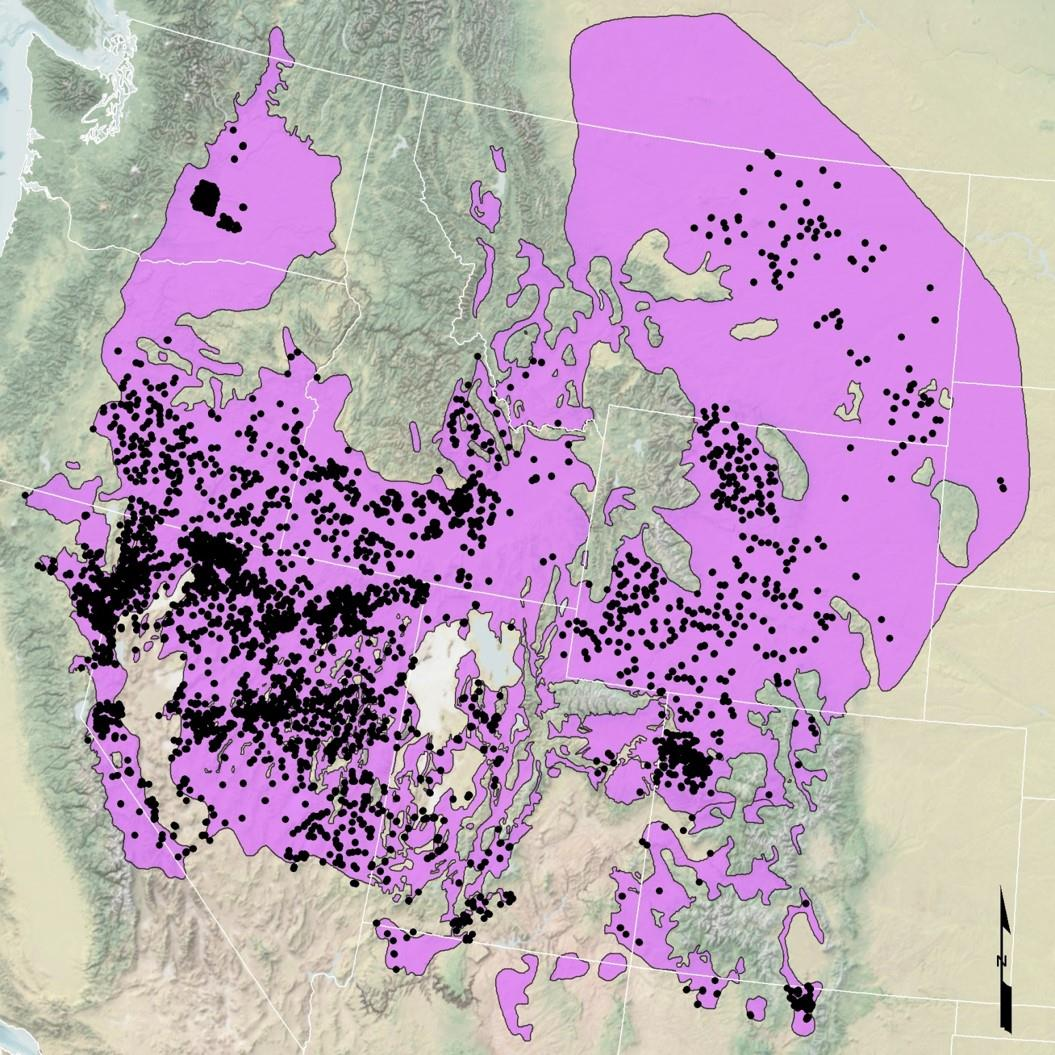
\includegraphics[width=\textwidth]{pics/studyarea.png}
 \caption{Study Region}\label{fig:studyarea}
\end{minipage}%
\begin{minipage}{.5\textwidth}
  \centering
  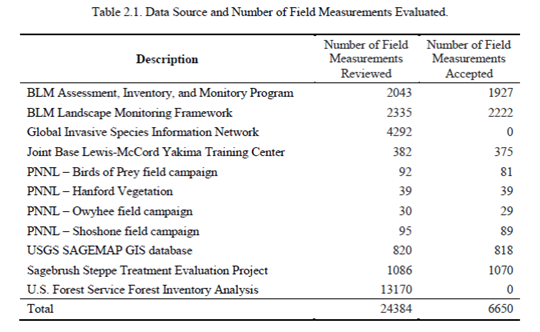
\includegraphics[width=\textwidth]{pics/fielddata.png}
\caption{Field Data}\label{fig:field}
\end{minipage}
\end{figure}
\subsection{Bio-physical Data}
Bio-physical datasets used for model development included the elevation, potential relative radiation index (PRR) (Pierce et al. 2005), and a growing degree day index.
Spatially interpolated climate data (precipitation, temperature) for the study area was acquired from the PRISM (Parameter-elevation Regressions on Independent Slopes Model) Climate Group (Daly et al. 1994; Daly et al. 2008; DiLuzio et al. 2008) and the Daily Surface Weather and Climatological Summaries (DAYMET) program (Thornton et al. 1997; Thornton et al. 2014). 
\subsubsection{Potential relative radiation}
 The PRR is a unitless index of available solar radiation for photosynthetic activity at a given location that takes into account the influence of geographic position, seasonal and daily variation in solar inclination, and topography. PRR was calculated by summing digital hillshade interpolations for a given period of interest as described by Pierce et al. (2005). Hourly hillshade interpolations were performed for daylight hours of one day of the month that most closely represents the average solar period for the month (i.e., PRR = Sum [Hillshadei-j, m-n], hours i-j for each representative day of months m-n). PRR calculated for use in this study reflects the solar conditions between October and June, which encompasses the bulk of the growing season of cheatgrass across the study area.
\begin{figure}
\centering
\begin{minipage}{.48\textwidth}
  \centering
  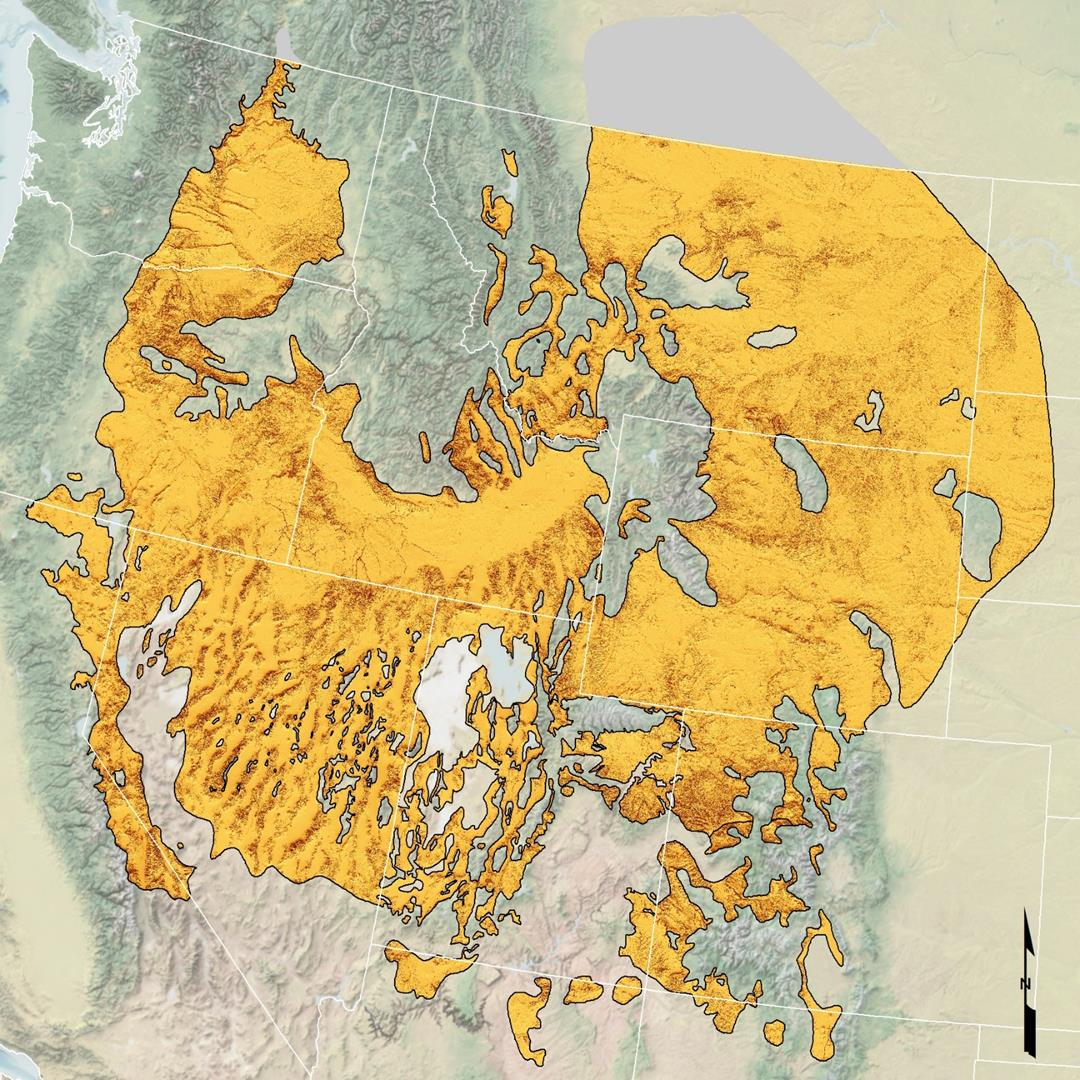
\includegraphics[width=\textwidth]{pics/prr.png}
 \caption{Potential Relative Radiation Index (light orange to dark orange illustrates high to low PRR).}\label{fig:prr}
\end{minipage}
\begin{minipage}{.04\textwidth}
\end{minipage}
\begin{minipage}{.48\textwidth}
  \centering
  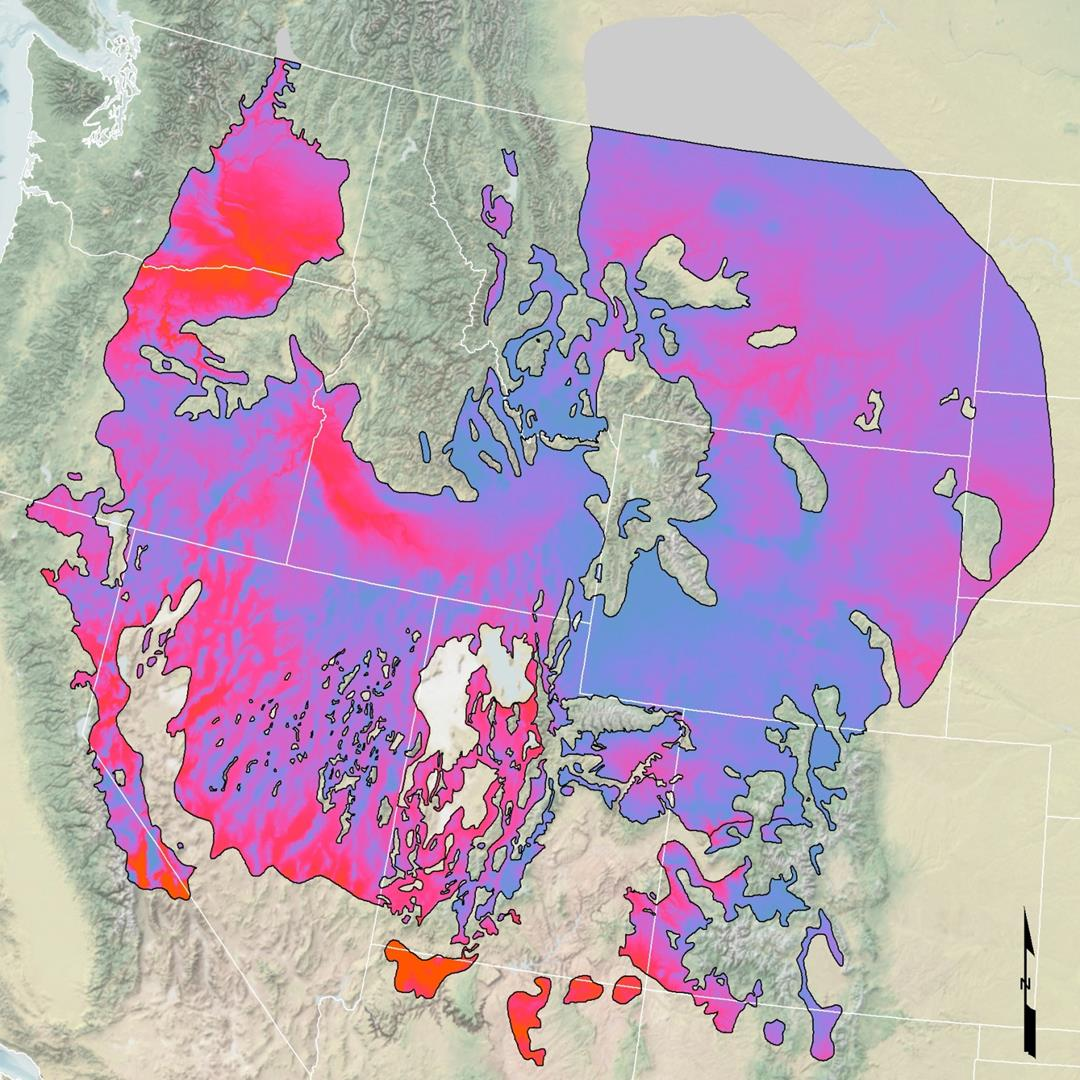
\includegraphics[width=\textwidth]{pics/gdd.png}
\caption{Cumulative Growing Degree Day (blue to red illustrates low to high GDD).}\label{fig:gdd}
\end{minipage}
\end{figure}

\subsubsection{DAYMET}
DAYMET provides gridded estimates of daily weather parameters for North America at a 1-km resolution, including daily continuous surfaces of minimum and maximum temperature and precipitation.
DAYMET daily minimum and maximum temperature data were acquired to calculated growing degree day index for the study area.
\subsubsection{Growing degree days}
Using the DAYMET daily minimum and maximum temperature data from 1 October 2014 to 30 April 2015, the cumulative growing degree day (GDD) index was calculated to represent the relative period of time when temperatures are suitable for plant growth (Figure 2.3). 
 
The cumulative GDD between October 1 and April 30 was calculated on a daily basis:
[(Tmax – Tmin)/2] – w
where w is the minimum temperature for growth of cheatgrass (assumed to be 0°C or 32°F), and summed for the period. Negative values were set to 0.

\subsubsection{PRISM}
PRISM uses point measurements of climate data and a digital elevation model of terrain to estimate continuous gridded surfaces of monthly climate elements at a 4-km resolution.  PRISM 30-year mean monthly and 30-year mean annual precipitation, minimum temperature, and maximum temperature (totaling 39 separate climate variables) were obtained to explore relationships between cheatgrass occurrence and general climate patterns. We also derived several seasonal cumulative precipitation and average minimum and maximum temperature variables from PRISM data that correspond to important seasonal periods during the life history of cheatgrass. 

\subsection{Ecological Data}
Our data set includes high level ecological data in the form  ecoregions, and land cover classification. 
\subsubsection{Ecoregions}
Ecoregions are areas which contain similar collections of plant and animal life, and similar ecological conditions such as geology, landforms, soils, vegetation, climate, land use, and water resources \cite{omernik2014ecoregions, salequzzaman2005ecoregions, ce1997ecological}.  
The study area spans 23 of the 182 level III ecoregions as defined by the U.S. Environmental Protection Agency (EPA) and the Commission for Environmental Cooperation (CEC). The ecoregion classifications for the study area were retrieved from the EPA hosted GIS data sets\footnote{\url{https://www.epa.gov/eco-research/ecoregions}}. Figure \ref{fig:ecoregion} shows the distributions of 16 ecoregions contained among the field measurement locations, while Table \ref{tab:ecomap} shows the distribution of ecoregions throughout the study area.
  \begin{figure}
  \begin{minipage}[b]{0.49\textwidth}
    \centering
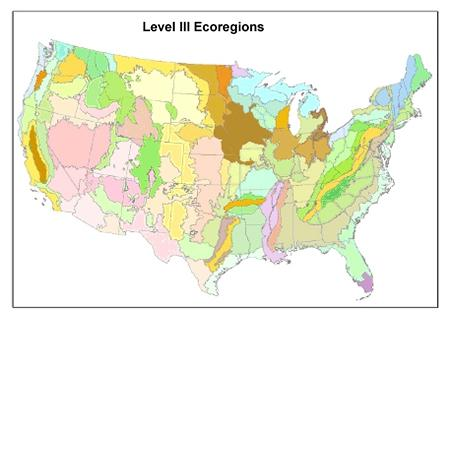
\includegraphics[width=\textwidth]{pics/ecoregions.jpg}
 \captionof{figure}{Figure from \url{https://www.epa.gov/eco-research/ecoregions}}\label{fig:ecoregion}
  \end{minipage}
  \hfill
  \begin{minipage}[b]{0.49\textwidth}
    \centering
   \begin{tabularx}{\linewidth}{l l r}
		\toprule[.2em]
		Region Number&\%&Region Name\\
		\midrule
		4&0&Cascades\\
		5&0&Sierra Nevada\\
		9&1.9&Eastern Cascades slopes and foothills\\
		10&8.7&Columbia plateau\\
		11&1.7&Blue Mountains\\
		12&9.3&Snake River plain\\
		13&36&Central basin and range\\
		15&0&Northern Rockies\\
		14&0&Mojave basin and range\\
		16&0.2&Idaho batholith\\
		17&1.2&Middle Rockies\\
		18&7.6&Wyoming basin\\
		19&0.3&Wasatch and Uinta Mountains\\
		20&3.7&Colorado plateaus\\
		21&0.02&Southern Rockies\\
		22&1.2&Arizona, New Mexico plateaus\\
		23&0&Arizona, New Mexico Mountains\\
		25&0.02&Wester high plains\\
		41&0&Canadian Rockies\\
		42&0.05&Northwestern glaciated plains\\
		43&2&Northwestern great plains\\
		77&0&North Cascades\\
		80&25.3&Northern basin and range\\ 
		\bottomrule[.2em]
	\end{tabularx}
      \captionof{table}{Study area ecoregions}\label{tab:ecomap}
    \end{minipage}

  \end{figure}

\subsubsection{LANDFIRE Landcover}
Categorical value for vegetation cover type generalized from LANDFIRE (www.landfire.gov) vegetation data. 15 classes.\\
\subsection{Satellite Imagery}\label{sat} For each location $i$ in the full study region, we have retrieved yearly and seasonal image data from the MODIS and LandSat platform and derived vegetation indexes.
\subsubsection{Normalized Difference Vegetation Index}
NDVI values provided by the LandSat \cite{usgs2014landsat} and MODIS platforms are calculated as a ratio between the red (R) and near infrared (NIR) values as:
\begin{equation}
\texttt{NDVI} = (\texttt{NIR} - \texttt{R}) / (\texttt{NIR} + \texttt{R})
\end{equation}
We define dNDVI as the peak NDVI (over a span of a year or a season) minus long-term median annual peak NDVI (across the years we have images for) .
\subsubsection{Enhanced Vegetation Index (EVI)}
EVI incorporates an “L” value to adjust for canopy background, “C” values as
coefficients for atmospheric resistance, and values from the blue band (B) in order to reduce the background noise, atmospheric noise, and saturation \cite{usgs2014landsat}.
\begin{equation}
\texttt{EVI} = \texttt{G} * ((\texttt{NIR} - \texttt{R}) / (\texttt{NIR} + \texttt{C}_1 * \texttt{R} - \texttt{C}_2 * \texttt{B} + \texttt{L}))
\end{equation}
\subsubsection{MODIS (annual, seasonal)} 
The MODIS annual and seasonal composite imagery data consists of 250m resolution pixel values associated with each study region location $i$. We have composite annual, spring, and summer pixel values for each location in the study area for each year from 2001-2016.  MODIS composite pixels are formed as the band or index value at the time of the peak NDVI value during the respective time range (spring, summer, or entire year).
Introducing some notation we define three matrices ${\bf M}_{\texttt{annual}}^{(i)}$, ${\bf M}_{\texttt{spring}}^{(i)}$, and ${\bf M}_{\texttt{summer}}^{(i)}$ for each study location $i$. Table \ref{tab:modis} shows the spectral bands and derived indices that form a each matrix  ${\bf M} \in \mathbb{R}^{16\times 7}$ of values with rows corresponding to the year, and columns corresponding to the spectral band or derived index. 
  \begin{figure}
  \begin{minipage}[b]{0.49\textwidth}
    \centering
\begin{tabularx}{\linewidth}{@{ }l X@{ }}
		\toprule[.2em]
		{\bf Column} &{\bf Band/Index} \\
		\midrule
		${\bf M}_{:,1}$& NDVI\\	
		${\bf M}_{:,2}$& EVI\\
		${\bf M}_{:,3}$& Blue (B)\\
		${\bf M}_{:,4}$& Red (R) \\
		${\bf M}_{:,5}$& Near Infra-Red (NIR)\\ 
		${\bf M}_{:,6}$& Mid Infra-Red (MIR)\\
		${\bf M}_{:,7}$& dNDVI\\
		\bottomrule[.2em]
	\end{tabularx}
 \captionof{table}{Columns for MODIS spectral bands and vegetation indexes.}\label{tab:modis}
  \end{minipage}
  \hfill
  \begin{minipage}[b]{0.49\textwidth}
    \centering
  \begin{tabularx}{\linewidth}{@{ }l X@{ }}
		\toprule[.2em]
		{\bf Column} &{\bf Band/Index} \\
		\midrule
		${\bf L}_{:,1}$& dNDVI\\
		${\bf L}_{:,2}$& Blue (B)\\
		${\bf L}_{:,3}$& Green (G) \\
		${\bf L}_{:,4}$& Red (R) \\
		${\bf L}_{:,5}$& Near Infra-Red (NIR)\\ 
		${\bf L}_{:,6}$& Short Wave Infra-Red 1 (SWIR1)\\ 
		${\bf L}_{:,7}$& Thermal, low gain channel  (T1)\\
		${\bf L}_{:,8}$& Thermal, high gain channel (T2)\\
		${\bf L}_{:,9}$& Short Wave Infra-Red 2 (SWIR2)\\
		\bottomrule[.2em]
	\end{tabularx}
      \captionof{table}{Columns for LandSat spectral bands and vegetation indexes.}\label{tab:landsat}
    \end{minipage}
  \end{figure}

\subsubsection{Landsat (annual, seasonal)}
The LandSat imagery differs from the MODIS imagery in resolution, spectral bands, years of operation, and composite product preparation. 
It consists of 30m resolution pixel values from the years 2003-2012. As in the case of MODIS, for convenience we define three matrices ${\bf L}_{\texttt{annual}}^{(i)}$, ${\bf L}_{\texttt{spring}}^{(i)}$, and ${\bf L}_{\texttt{summer}}^{(i)}$ for each study location $i$.  Table \ref{tab:landsat} shows the spectral bands and derived indices that form a each matrix  ${\bf L} \in \mathbb{R}^{10\times 9}$ of values with rows corresponding to the year, and columns corresponding to the spectral band or derived index. 

\subsection{Data Synopsis}
 Tables \ref{tab:targets}, \ref{tab:cat}, and \ref{tab:data} contain brief descriptions of all variables used in modeling cheatgrass coverage. 
The complete set of data used in training predictive mapping models consists of 6602 locations with available field measurements due to missing values from 49 data points in the original data set. 
We define, ${\bf w} \in \mathbb{N}^{6602 \times 1}$ as the matrix of unique integer ids for each data point, 
${\bf y} \in \mathbb{R}^{6602 \times 1}$, where  ${\bf y }_{i,1} = y^{(i)}_1$the matrix of coverage values for each data-point, 
${\bf C} \in \mathbb{R}^{6602\times 3}$, where  ${\bf C }_{i,j} = c^{(i)}_j$ the matrix of categorical variables associated 
with each data point, and ${\bf X} \in \mathbb{R}^{6602\times 664}$, 
where  ${\bf x }_{i,j} = x^{(i)}_j$. 
These values $\begin{bmatrix} {\bf w} & {\bf y} & {\bf C} & {\bf X}\end{bmatrix}$ are stored in comma delimited plain text csv format and may be accessed at \url{http://tobedetermined.gov}.
\begin{table}
\begin{tabularx}{\linewidth}{@{ }l X@{ }}
\toprule[.2em]
{\bf Variable} &{\bf Description} \\
\midrule
$y_p$ & Proportion (0-1) of cheat cheat grass cover. \\
 $y_c$ &Cover class. 0 if $y_r \leq 0.2$, 1 otherwise.\\
\bottomrule[.2em]
\end{tabularx}
\caption{Prediction Targets} \label{tab:targets}
\end{table}

\begin{table}
\begin{tabularx}{\linewidth}{@{ }l X@{ }}
\toprule[.2em]
{\bf Variable} &{\bf Description} \\
\midrule
$c_1$ & Soil temperature and moisture regime class value. \\
$c_2$ & Categorical value for vegetation cover type generalized from LANDFIRE (www.landfire.gov) vegetation data. 15 classes.\\
$c_3$ & EPA Level III Ecoregions.\\	
\bottomrule[.2em]
\end{tabularx}
\caption{Categorical Variables} \label{tab:cat}
\end{table}

\begin{table}
\begin{tabularx}{\linewidth}{@{ }l X@{ }}
\toprule[.2em]
{\bf Variable} &{\bf Description} \\
\midrule
$x_1$ & Latitude.\\
$x_2$ & Longitude. \\
\cellcolor[gray]{0.9}$x_3$ & \cellcolor[gray]{0.9}Elevation above sea level.\\
\cellcolor[gray]{0.9}$x_4$ & \cellcolor[gray]{0.9}Potential Relative Radiation (available solar radiation for photosynthesis).\\
$x_{5}$ & Long-term median cumulative winter precipitation based on PRISM.\\
$\cellcolor[gray]{0.9}x_{6}$ & \cellcolor[gray]{0.9}Long-term median cumulative growing degree days (GDD), Oct-Apr.\\
$\cellcolor[gray]{0.9}x_{7:18}$ & \cellcolor[gray]{0.9}Normal 30 year monthly max temperatures. Original study used month 5.\\
$x_{19}$ & 30-year normal annual maximum temperature.\\
$\cellcolor[gray]{0.9}x_{20:31}$ & \cellcolor[gray]{0.9}30-year normal monthly min temperatures. Original study used months 3,11.\\
$x_{32}$ & 30-year normal annual minimum temperature.\\
$\cellcolor[gray]{0.9}x_{33:44}$ & \cellcolor[gray]{0.9}30-year normal monthly precipitation for all months. Original study used months 3,6,7.\\
$x_{45}$ & 30-year normal annual precipitation.\\
$\cellcolor[gray]{0.9}x_{46}$ &\cellcolor[gray]{0.9} Average of 30-year normal monthly maximum temperature during select winter months (Nov-Feb)\\
$\cellcolor[gray]{0.9}x_{47}$ &\cellcolor[gray]{0.9} Cumulative precipitation during select winter season months (Dec-Feb).\\
$x_{48}$ & Cumulative precipitation during select spring season months (Apr-May).\\
$x_{49}$ & Cumulative precipitation during select  summer season months (Jun-Sep).\\
$x_{50}$ & 30-year normal monthly minimum temperature during select winter months (Nov-Dec).\\
%$\cellcolor[gray]{0.9}x_{51}$&\cellcolor[gray]{0.9}MODIS long-term median annual peak NDVI.\\
\cellcolor[gray]{0.9}$x_{52}$ & \cellcolor[gray]{0.9}Delta NDVI (Normalized Difference Vegetation Index) from long term median peak NDVI in year of peak cumulative winter precipitation.\\
$x_{53}$&Landsat7 long-term median annual peak NDVI.\\
$x_{54}$&Landsat7 long-term median spring peak NDVI.\\
$x_{55}$&Landsat7 long-term median summer peak NDVI.\\
$x_{56:325}$ &  LandSat annual, spring, summer composite pixels.\\
$x_{326:661}$ & MODIS annual, spring, summer composite pixels.\\
$x_{662}$ &  MODIS annual peak NDVI.\\
$x_{663}$ & MODIS spring peak NDVI\\
$x_{664}$ & MODIS summer peak NDVI.\\
\bottomrule[.2em]
\end{tabularx}
\caption{Continuous Variables. Shaded variables were used in making the original Linear Discriminant Analysis model.} \label{tab:data}
\end{table}
%============================================================================================
%============================================================================================
%Section: Methods================================================
%=============================================================================================
%============================================================================================
\section{Methods}
In our search for prospective models for producing high quality predictive maps at finest resolution across the full range of our study area, we explored classification models for the presence of cheatgrass. For the categorical mapping of cheatgrass
occurrence, we chose two cover classes based on an evident separation in cheatgrass cover in the field
data: $≤ 2\%$ (low cover or absent) or cover $> 2\%$ (high cover or present \ref{fig:cov}. 
%Use of these classes provided better ability to distinguish cheatgrass with respect to the variables included in the model. 
The location of field points colored by these classifications is shown in Figure \ref{fig:covclass}. Continuous variables used in model development were standardized by subtracting the mean and then dividing
by the standard deviation. 
\begin{figure}
\centering
\begin{minipage}{.48\textwidth}
  \centering
  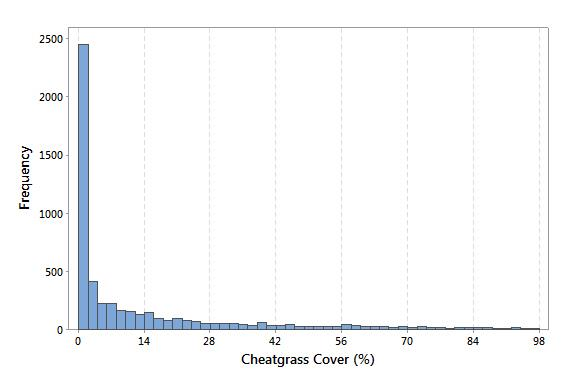
\includegraphics[width=\textwidth]{pics/cov.png}
 \caption{Histogram Showing Distribution of Cheatgrass Cover Values Measured at Field Locations.}\label{fig:cov}
\end{minipage}
\begin{minipage}{.04\textwidth}
\end{minipage}
\begin{minipage}{.48\textwidth}
  \centering
  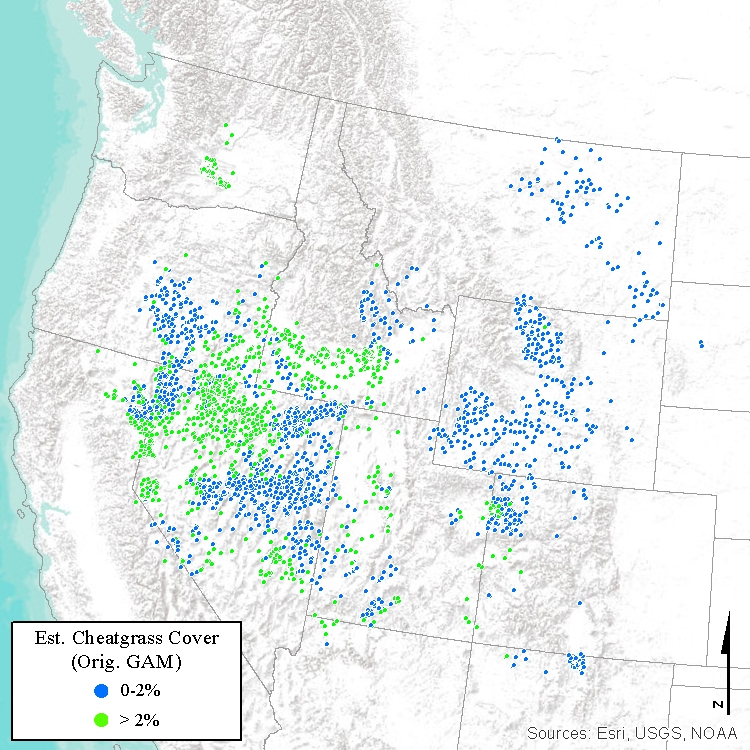
\includegraphics[width=\textwidth]{pics/field_samp_3Mar2016_oGAM_covclass.jpg}
\caption{Classification of field samples}\label{fig:covclass}
\end{minipage}
\end{figure}



\subsection{Baseline Models}
For this study we explored two baseline methods for classification, Random Forest (RF), and Linear Discriminant Analysis (LDA). 
%We also explored two regression models, linear regression and a Random Forest regressor. 
We chose LDA as a baseline model for comparison of the current approach to prior work on mapping cheatgrass with a linear model using satellite imagery. Random Forest was chosen as it has competitive performance with deep learning models in low resource data regimes as is the case of our 6,000 field locations. We used the implementation of Random Forest and Linear Discriminant Analysis  provided in the Sci-kit learn python library.

%D1
%{'bootstrap': True, 'min_samples_leaf': 4, 'n_estimators': 136, 'max_features': 'sqrt', 'min_samples_split': 5, 'max_depth': 80}
%0.808974758492
%D2
%{'bootstrap': False, 'min_samples_leaf': 4, 'n_estimators': 178, 'max_features': 'auto', 'min_samples_split': 2, 'max_depth': 50}
%0.814116547211
%D3
%{'bootstrap': False, 'min_samples_leaf': 1, 'n_estimators': 157, 'max_features': 'sqrt', 'min_samples_split': 5, 'max_depth': 70}
%0.827360548457
%D4
%{'bootstrap': False, 'min_samples_leaf': 4, 'n_estimators': 200, 'max_features': 'auto', 'min_samples_split': 2, 'max_depth': 60}
%0.826425677781
%============================================================================================
% Subsection Deep Learning Models================================================
%=============================================================================================
\subsection{Deep Learning Models}
Deep learning models were chosen as prospective modeling candidates due to their potential for mapping high dimensional input features (such as our 664 continuous variables and 3 categorical values) into a lower dimensional representation which captures the inherent relationships between variables to greatest effect. The final layer of our deep learning models is the same transformation that is learned for logistic regression in the case of classification.
% and linear regression in the case of regression predictions. 
A convenient way to view a deep learning model in our context is that it learns a parametrized non-linear mapping from input variables to a latent variable which is then used as input to a linear model. The parameters of the non-linear mapping and ultimate linear model are fit jointly, end to end using the ADAM variant of stochastic gradient descent. 

We define the inputs to the neural network as a real valued vector $\widehat{{\bf x}}^{(i)}$ , it's predictions $\widehat{{\bf y}}^{(i)}\in \mathbb{R}^2$, a probability distribution over 2 classes, and the ground truth for a field location as ${\bf y}^{(i)}$. Since we are interested in an ablative analysis of the contributions in modeling performance from using data from satellite platforms jointly and independently we define subsets on the full set of continuous variables defined as ${\bf x}$ in Table \ref{tab:data}:
\begin{eqnarray}\label{eqn:subset}
D_1({\bf x}) &= {\bf x}_{1:50}\hspace{50pt}&\textrm{Biophysical variables}\\
D_2({\bf x})  &= {\bf x}_{1:50,326:664}\hspace{50pt}&\textrm{Biophysical varibles + MODIS}\\
D_3({\bf x})  &= {\bf x}_{1:325}\hspace{50pt}&\textrm{Biophysical varibles + LandSat}\\
D_4({\bf x}) &= {\bf x}\hspace{50pt}&\textrm{All variables}\\\label{eqn:subset2}
\end{eqnarray}

Since our data contains categorical variables derived from ecological analysis which we wish to incorporate into the model we define three learned embedding matrices for the categorical variables, ${\bf W}_{\texttt{cover}}\in \mathbb{R}^{15 \times k}$, ${\bf W}_{\texttt{eco}}\in \mathbb{R}^{23 \times k}$, and ${\bf W}_{\texttt{soil}}\in \mathbb{R}^{9 \times k}$, corresponding to the 15 classes of derived generalized LANDFIRE cover classes, the 23 level III ecoregions, and the 9 soil temperature and moisture regime class values exhibited in the full study region. The rows of these matrices correspond to classes for their respective categories. The number of columns $k$ is the size of the embedding vector for a class; a so called hyperparameter or modeling choice. These embedding vectors are learned jointly with the other parameters of the neural network. Our input to a prospective neural network model is then defined using block matrix notation as:
\begin{equation}
\widehat{{\bf x}}^{(i)} = \begin{bmatrix}{\bf c}_1^{(i)}{\bf W}_{\texttt{soil}}&{\bf c}_2^{(i)}{\bf W}_{\texttt{cover}}&{\bf c}_3^{(i)}{\bf W}_{\texttt{eco}}&D_*\bigl({\bf x}^{(i)}\bigr)\end{bmatrix}
\end{equation}
where ${\bf c}_1^{(i)}$, ${\bf c}_3^{(i)}$, and ${\bf c}_3^{(i)}$ are so called one hot representations\footnote{A one hot class vector representation has a number of elements equal to the number of classes with a 1 for the class represented and 0 everywhere else} of soil, land cover, and ecoregion class respectively, and $D_*\bigl({\bf x}^{(i)}\bigr)$ is one of the four subsets of continuous variables defined in Equations \ref{eqn:subset}$-$\ref{eqn:subset2}. The row vector matrix multiplications select the embedding vector associated with a particular class so that it can be concatenated to the rest of the continuous variables in the neural network input. For simplicity of notation the rest of discussion for deep learning model development we will omit subscripts $i$.
%============================================================================================
% Subsubsection DNN================================================
%=============================================================================================
\subsubsection{Deep Neural Network}\label{dnn}
Particular deep neural network (DNN) configurations for classification and regresssion are depicted in Figure \ref{fig:dnn}. The model consists of $L$ hidden layers ${\bf h}_l$ which are recursively defined as:

\begin{eqnarray}
{\bf h}_l &= &\texttt{RELU}({\bf W}_l {\bf h}_{l-1} + {\bf b}_l)\\
{\bf h}_0&=&\widehat{{\bf x}}
\end{eqnarray}

where the nonlinear \texttt{RELU} operation is defined as the elementwise vector valued operation:
\begin{equation}
\texttt{RELU}({\bf x})_i = \texttt{max}({\bf x}_i, 0)
\end{equation}


The output of the DNN maps the final hidden representation ${\bf h}_L$ to a probability distribution over cheatgrass occurence classes of the form:
\begin{equation}
\widehat{{\bf y}} = \texttt{softmax}({\bf W}_{L+1}{\bf h}_L + {\bf b}_{L+1})
\end{equation}

where the \texttt{softmax} operation is defined as the elementwise vector valued operation:
\begin{equation}
\texttt{softmax}({\bf x})_i = \frac{e^{{\bf x}_i}}{\sum_{j}e^{{\bf x}_j}}
\end{equation}

The parameters ${\bf W}$, ${\bf b}$ are optimized using stochastic gradient descent with the objective function being the cross-entropy loss between the predicted class distribution $\widehat{{\bf y}}$ and true class distribution ${\bf y}$. Beyond this basic formulation we also employ dropout for normalization to aviod overfitting and batch normalization for better conditioned gradient updates. 
%============================================================================================
% Subsubsection RNN================================================
%=============================================================================================
\subsubsection{Recurrent Neural Network}
A deep neural network as described in \ref{dnn} has the potential as a universal function approximator to model cheatgrass distribution given the field data with an optimal Bayes error. In practice however, since the optimal function may be difficult to find during the optimization we developed a joint recurrent neural network (RNN) model intended to take greater advantage of the time series implicit in the satellite imagery data. In this section we detail a model for fusing time series of data from different satellite platforms into a latent representation that can be used for linear classification. The model consists of two separate bidirectional RNNs which model time series of the MODIS and LandSat derived imagery products respectively. 
A particular instantiation of this modeling approach is depicted in Figure \ref{fig:rnn}. More formally we define two bidirectional Long Short Term Memory networks  which are operations on sequences of pixel vectors from the MODIS and LandSat platforms respectively,  $\texttt{LSTM}_{\texttt{MOD}}(\mathcal{X})$ and  $\texttt{LSTM}_{\texttt{LAN}}(\mathcal{X})$. Given a seqence of vectors $\mathcal{X}$ each LSTM outputs a condensed vector representation of the time series. The time series for the MODIS and LandSat data consist of sequences of 16, and 10 vectors respectively, one for each year that pixel values were obtained. From the notation developed in \ref{sat}, the $t$-th vector in the LandSat series is:
\begin{equation}{\bf \mathcal{X}}^{\texttt{LAN}}_{t} =
\begin{bmatrix}{\bf L}^{\texttt{annual}}_{t,1}& ....& {\bf L}^{\texttt{annual}}_{t,10}&{\bf L}^{\texttt{spring}}_{t,1}& ....& {\bf L}^{\texttt{spring}}_{t,10}& {\bf L}^{\texttt{summer}}_{t,1}& ...& {\bf L}^{\texttt{summer}}_{t,10}\end{bmatrix}
\end{equation}
whereas the $t$-th vector in the MODIS time series is:
\begin{equation}{\bf \mathcal{X}}^{\texttt{MOD}}_{t} =
\begin{bmatrix}{\bf M}^{\texttt{annual}}_{t,1}& ....& {\bf M}^{\texttt{annual}}_{t,10}&{\bf M}^{\texttt{spring}}_{t,1}& ....& {\bf M}^{\texttt{spring}}_{t,10}& {\bf M}^{\texttt{summer}}_{t,1}& ...& {\bf M}^{\texttt{summer}}_{t,10}\end{bmatrix}
\end{equation}

These resulting representation vectors are concatenated with the categorical embeddings and the continuous biophysical variables for the input to a deep neural network as described in \ref{dnn} where:
\begin{equation}
\widehat{{\bf x}} = \begin{bmatrix}{\bf c}_1{\bf W}_{\texttt{soil}}&{\bf c}_2{\bf W}_{\texttt{cover}}&{\bf c}_3{\bf W}_{\texttt{eco}}&D_1 \bigl({\bf x}\bigr) &\texttt{LSTM}_{\texttt{MOD}}\bigl(\mathcal{X}^{\texttt{MOD}}\bigr)&\texttt{LSTM}_{\texttt{LAN}}\bigl(\mathcal{X}^{\texttt{LAN}}\bigr)\end{bmatrix}
\end{equation}

\begin{figure}
\centering
\begin{minipage}{.48\textwidth}
  \centering
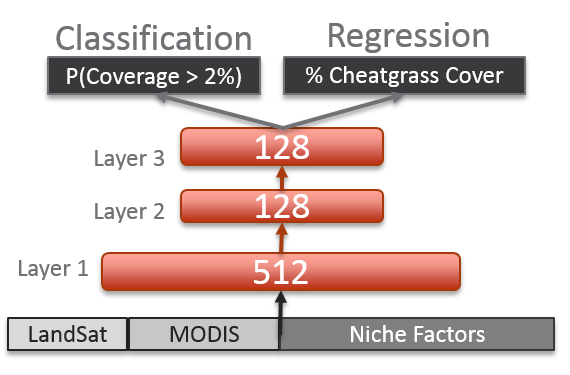
\includegraphics[width=\textwidth]{pics/dnn.png}
\caption{Deep Neural Network for Classification}\label{fig:dnn}
\end{minipage}
\begin{minipage}{.04\textwidth}
\end{minipage}
\begin{minipage}{.48\textwidth}
  \centering
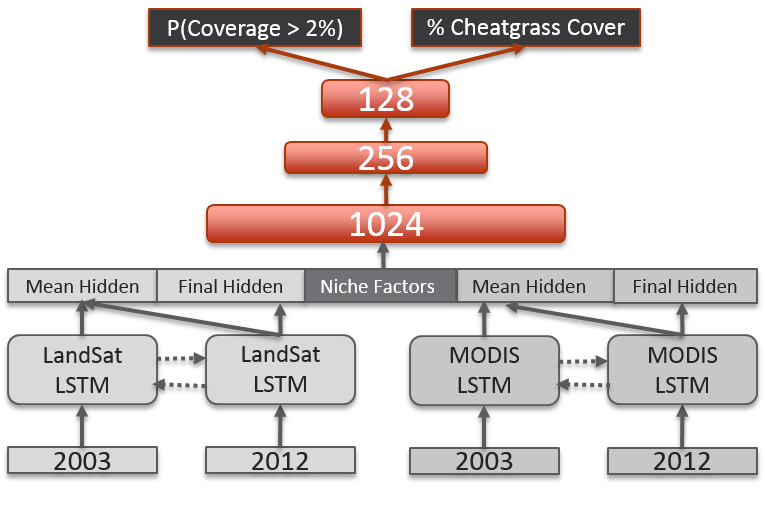
\includegraphics[width=\textwidth]{pics/rnn.png}
\caption{Recurrent Neural Network for Classification}\label{fig:rnn}
\end{minipage}
\end{figure}
%============================================================================================
% Subsection Experimental Setup================================================
%=============================================================================================
\subsection{Experimental Setup}
In order to gage the effectiveness of incorporating satellite data from multiple platforms we trained each prospective model on each of four subsets of the complete data. For the neural network models we also include the categorical variables for each subset of the data. 
\begin{itemize}
	\item $D_1$: Ecological Niche Factors 
	\item $D_2$:  Ecological Niche Factors + MODIS imagery
	\item $D_3$:  Ecological Niche Factors + LandSat imagery
	\item $D_4$: All Variables.
\end{itemize} 
We performed a random hyperparameter search for each prospective model. For each model we chose 200 random configurations of hyperparameters within reasonable ranges for performance and computation time. For each of these runs we tested performance using 5-fold stratified cross-validation where field data was split  into each of the 5 folds with equal distributions over the different ecoregions and generalized land cover classifications. 
%============================================================================================
%============================================================================================
%Section: Results and Analysis================================================
%=============================================================================================
%============================================================================================
\section{Results and Analysis}
In this section we discuss the results of experiments and analyze the model predictions for the final mapping product. In section \ref{sec:res1} we discuss performance of all models trained for the field locations in the dataset. Following this discussion we perform a detailed ablation analysis for the described subsets of variables on the best performing model. To this end we first discuss training statistics for models from each variable subset, performing an ablation analysis on key training statistics. We then look more closely at the classification performance to assess potential weaknesses in the prospective model by analysis of predictions versus true class considering high level derived variables such as ecoregion, coverage class and soil regime. Finally, we shift our focus to analysis and assessment of the complete mapping product derived from the highest performing model, with specific focus on the variation of confidence for various points in the full study region that were not present in the training data. 
%============================================================================================
% Subsection Performance on Field measurement locations================================================
%=============================================================================================
\subsection{Performance on Field measurement locations}
In this section we report statistics on field measurement locations.
\subsubsection{Quantitative assessment} \label{sec:res1}
Quantitative results are reported for the average performance across cross-validation folds for each of the 4 subsets of input variables. Table \ref{tab:perf2} shows the outcomes of experiments in terms of accuracy for classification prediction. 
The best performing subset of input variables is bolded in each row of the tables, while the best overall performing model, the DNN using all available input data is highlighted in red. We note a a few trends. Incorporating satellite data of either form leads to better results. In addition, Random forest and LDA do not gain any advantage from incorporating both MODIS and LandSat imagery whereas the neural network models improve in accuracy from incorporating imagery from both platforms. Finally, we note that the recurrent neural network did not perform as well as the DNN, possibly due to the larger number of parameters to be fit on the same number of data points.

We chose the best performing model in terms of accuracy (DNN with all input variables) to create the final mapping product, and for this model we report several classification statistics for each of the four input variable subsets in Table \ref{tab:dnnperf}. Here we the same trend for recall, F-score, and area under the ROC curve in that adding imagery from either sattellite platform gives the most significant improvement, with the LandSat imagery demonstrating more improvement. The best results for all these metrics are once again from the inclusion of imagery from both satellite platforms. 
  \begin{figure}
  \begin{minipage}[b]{0.49\textwidth}
    \centering
 \begin{tabularx}{\linewidth}{l r r r r r}
		\toprule[.2em]
		 &$D_1$& $D_2$&$D_3$&$D_4$\\
		\midrule
		{\bf LDA}&73.816 & 78.279&{\bf 80.653} &79.826\\
		{\bf RF}&80.165 &81.677&82.502 &{\bf 82.798}\\
		{\bf DNN}&79.604& 82.004&82.456 &\textcolor{red}{\bf 83.203}\\
		{\bf RNN}&--- & 81.388&81.820 &{\bf 82.707}\\
		\bottomrule[.2em]
	\end{tabularx}
	\captionof{table}{Classification accuracy of models for subsets of data} \label{tab:perf2}
    \end{minipage}
\hfill
  \begin{minipage}[b]{0.49\textwidth}
    \centering
%\begin{tabularx}{\linewidth}{l r r r r r}
%		\toprule[.2em]
%		 &$D_1$ &$D_2$&$D_3$&$D_4$\\
%		\midrule
%		{\bf LR}&0.1340  & 0.1115&{\bf 0.1041} &0.1059\\
%		{\bf RF}& 0.0913  &0.0926&0.0909 &{\bf 0.0909}\\
%		{\bf DNN}&0.1006  &0.0795&0.0787 &\textcolor{red}{\bf 0.0746}\\
%		{\bf RNN}&---  & 0.0790&0.0806 &{\bf 0.0766}\\
%		\bottomrule[.2em]
%	\end{tabularx}
%	\captionof{table}{Mean Absolute Error for predicting cheat grass coverage.} \label{tab:perf3}
\begin{tabularx}{\linewidth}{l r r r r r r}
		\toprule[.2em]
		 &{\bf Prec.}& {\bf Rec.}&{\bf F-scr}&{\bf AUC}&{\bf Acc.}&{\bf Std.}\\
		\midrule
		$D_1$&0.795& 0.820&0.808 &0.866&0.796&0.025\\
		$D_2$&0.844 &0.803&0.823 &0.893&0.820&0.014\\
		$D_3$&0.831& 0.833&0.832 &0.900&0.825&0.015\\
		$D_4$&0.837& 0.842&0.839 &0.902&0.832&0.012\\
		\bottomrule[.2em]
	\end{tabularx}
	\captionof{table}{Performance across a range of metrics for most accurate DNN models for each subset of input variables. The last column reports the standard deviation of the accuracy across different cross-validation folds.} \label{tab:dnnperf}
  \end{minipage}
 
  \end{figure}

 \begin{figure}
  \begin{minipage}[b]{0.49\textwidth}
    \centering

\begin{tabularx}{\linewidth}{l r r r r r r}
		\toprule[.2em]
		 &{\bf Prec.}& {\bf Rec.}&{\bf F-scr}&{\bf AUC}&{\bf Acc.}&{\bf Std.}\\
		\midrule
		$D_1$&--& --&-- &--&--&--\\
		$D_2$&-- &--&--- &---&---&---\\
		$D_3$&---& ---&--- &---&---&---\\
		$D_4$&0.830& 0.840&0.835 &0.904&0.827&0.011\\
		\bottomrule[.2em]
	\end{tabularx}
	\captionof{table}{Performance across a range of metrics for most accurate RNN models for each subset of input variables. The last column reports the standard deviation of the accuracy across different cross-validation folds.} \label{tab:dnnperf}
    \end{minipage}
\hfill
  \begin{minipage}[b]{0.49\textwidth}
    \centering




\begin{tabularx}{\linewidth}{l r r r r r r}
		\toprule[.2em]
		 &{\bf Prec.}& {\bf Rec.}&{\bf F-scr}&{\bf AUC}&{\bf Acc.}&{\bf Std.}\\
		\midrule
		$D_1$&0.807& 0.815&0.811 &0.883&0.802&0.024\\
		$D_2$&0.825 &0.823&0.824 &0.891&0.816&0.024\\
		$D_3$&0.827& 0.838&0.833 &0.901&0.825&0.021\\
		$D_4$&0.835& 0.835&0.835 &0.904&0.828&0.025\\
		\bottomrule[.2em]
	\end{tabularx}
	\captionof{table}{Performance across a range of metrics for most accurate RF models for each subset of input variables. The last column reports the standard deviation of the accuracy across different cross-validation folds.} \label{tab:dnnperf}
  \end{minipage}
 
  \end{figure}
%\begin{table}
%\begin{tabularx}{\linewidth}{l r r r r r r}
%		\toprule[.2em]
%		 &{\bf Precision}& {\bf Recall}&{\bf F-score}&{\bf AUC}&{\bf Accuracy}&{\bf Std. Accuracy}\\
%		\midrule
%		$D_1$&0.795& 0.820&0.808 &0.866&0.796&0.025\\
%		$D_2$&0.844 &0.803&0.823 &0.893&0.820&0.014\\
%		$D_3$&0.831& 0.833&0.832 &0.900&0.825&0.015\\
%		$D_4$&0.837& 0.842&0.839 &0.902&0.832&0.012\\
%		\bottomrule[.2em]
%	\end{tabularx}
%	\caption{Performance across a range of metrics for most accurate DNN models for each subset of input variables.} \label{tab:dnnperf}
%\end{table}

%================================
% Subsubsection Training Statistics
%================================
\subsubsection{Training Statistics}
In this section we analyse training statistics for the best performing model. We first look at plots of train versus test performance for the best performing cross-validation fold for each of the input variable subsets. Looking at several different metrics we see training is noisier and has a greater tendency to overfit with inclusion of the modis data. Conversely we see that incorporating the LandSat data into the model has a regularizing effect which limits the amount of overfitting so that test performance converges closer to train performance. We also consider the dropout probability for each data subset (for each model run a random dropout probability was selected to be between 0.5 and 1.0. Table \ref{drop} shows the dropout probabilities and hidden layer sizes for the different data subsets. The columns for using MODIS only or LandSat show that these models have comparable dropout probabilities and network size. The MODIS only input model does have the largest network which greatens the chance of overfitting but a large dropout probability which should have more of a regularizing effect. A more careful analysis with identical sized networks and dropout probabilities would confirm what the present analysis suggests (that the MODIS data has some properties which encourage overfitting). With careful use of early stopping we can see in figure 53 that the best loss  can in fact be achieved by incorporating all the data. 

\begin{table}
\begin{tabularx}{\linewidth}{l r r r r}
		\toprule[.2em]
		 &{\bf $D_1$}& {\bf $D_2$}&{\bf $D_3$}&{\bf $D_4$}\\
		\midrule
		Dropout Probability&0.275&0.350& 0.30&.5\\
		Layer 1&256&256& 256&256\\
		Layer 2&256&256&64&32\\
		Layer 3&64&128&256&256\\
		\bottomrule[.2em]
	\end{tabularx}
	\caption{Hyperparameters for most accurate DNN models for each subset of input variables.} \label{tab:dnnhyper}
\end{table}
%d1 dp 7.25 256 256 64
%d2 dp 0.65 256 256 128
%d3 dp 0.7 256 64 256
%d4 dp .5 256 32 256
%================================
% Subsubsection Best Training Statistics
%================================
% Accuracy Train versus test
%best
\begin{figure}
\centering
\begin{minipage}{.24\textwidth}
  \centering
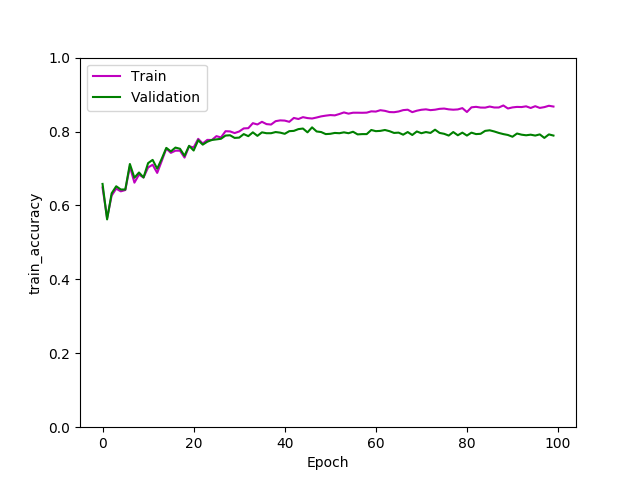
\includegraphics[width=\textwidth]{pics/d1_train_accuracy_best_train_test.png}
\caption{$D_1$}\label{fig:d1acctraintest}
\end{minipage}
\begin{minipage}{.01\textwidth}
\end{minipage}
\begin{minipage}{.24\textwidth}
  \centering
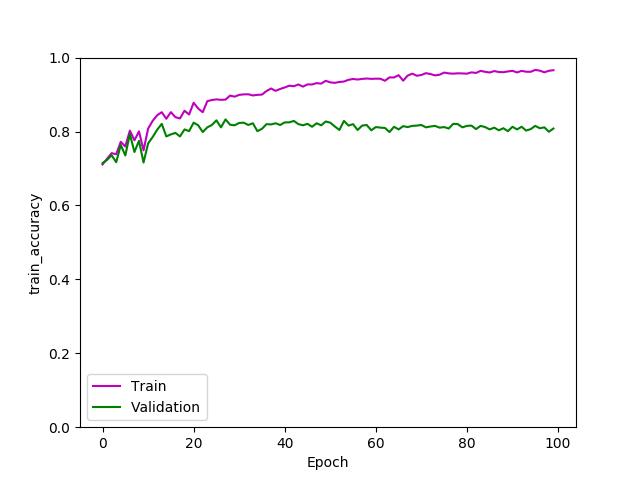
\includegraphics[width=\textwidth]{pics/d2_train_accuracy_best_train_test.png}
\caption{$D_2$}\label{fig:d2acctraintest}
\end{minipage}
\begin{minipage}{.24\textwidth}
  \centering
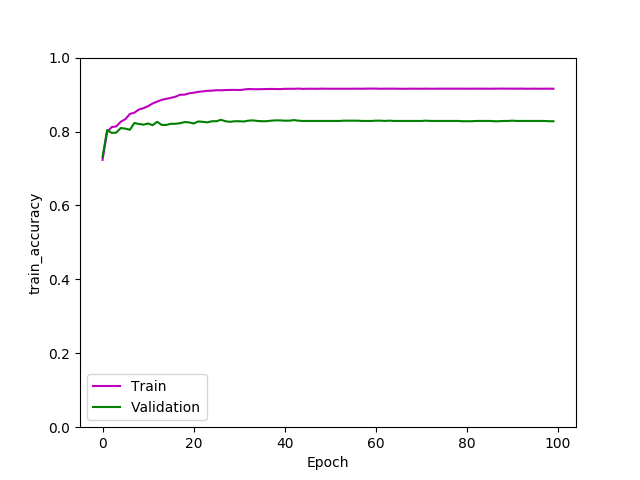
\includegraphics[width=\textwidth]{pics/d3_train_accuracy_best_train_test.png}
\caption{$D_3$}\label{fig:d3acctraintest}
\end{minipage}
\begin{minipage}{.01\textwidth}
\end{minipage}
% average
\begin{minipage}{.24\textwidth}
  \centering
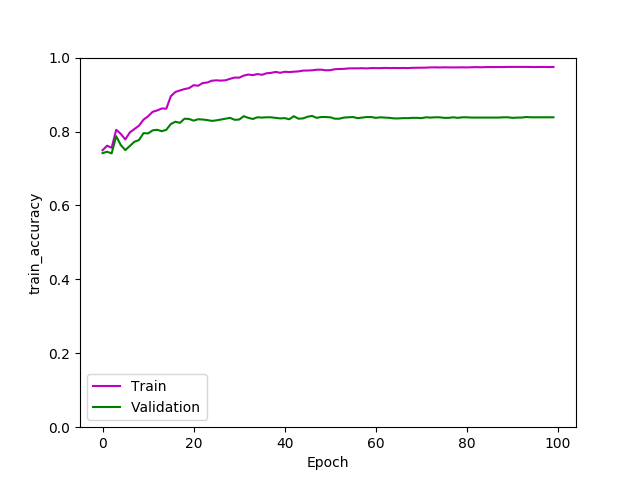
\includegraphics[width=\textwidth]{pics/d4_train_accuracy_best_train_test.png}
\caption{$D_4$}\label{fig:d4acctraintest}
\end{minipage}
\caption{Train versus test accuracy for the best performing cross-validation fold for input variable subsets}\label{fig:traintestacc}
\end{figure}
\begin{figure}
\centering
\begin{minipage}{.24\textwidth}
  \centering
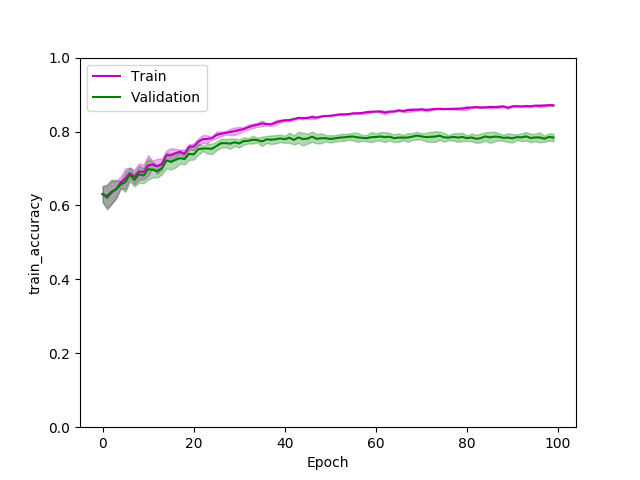
\includegraphics[width=\textwidth]{pics/d1_train_accuracy_mean_train_test.png}
\caption{$D_1$}\label{fig:d1acctraintest}
\end{minipage}
\begin{minipage}{.01\textwidth}
\end{minipage}
\begin{minipage}{.24\textwidth}
  \centering
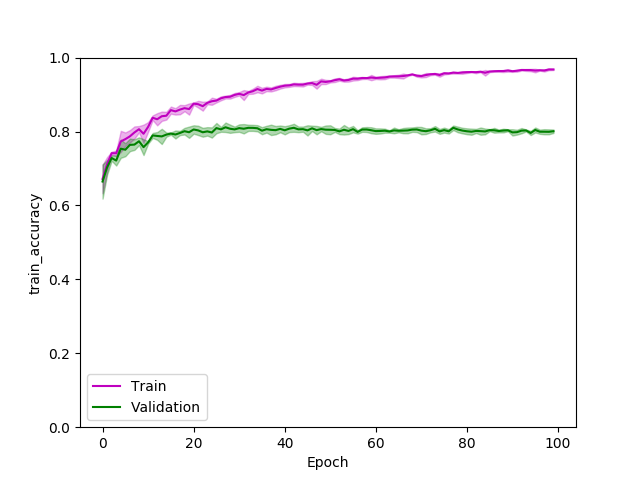
\includegraphics[width=\textwidth]{pics/d2_train_accuracy_mean_train_test.png}
\caption{$D_2$}\label{fig:d2acctraintest}
\end{minipage}
\begin{minipage}{.24\textwidth}
  \centering
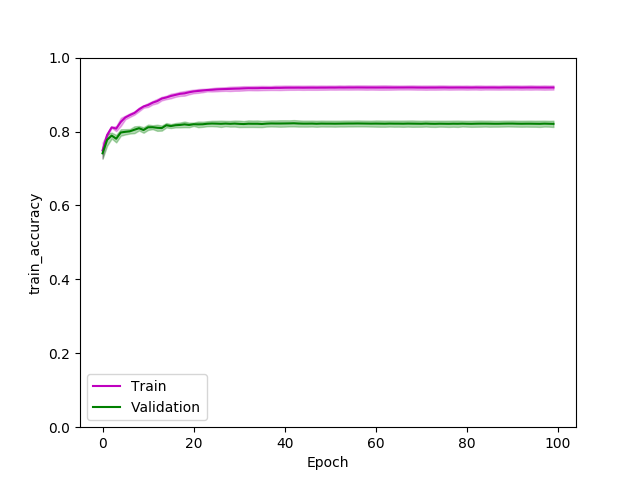
\includegraphics[width=\textwidth]{pics/d3_train_accuracy_mean_train_test.png}
\caption{$D_3$}\label{fig:d3acctraintest}
\end{minipage}
\begin{minipage}{.01\textwidth}
\end{minipage}
\begin{minipage}{.24\textwidth}
  \centering
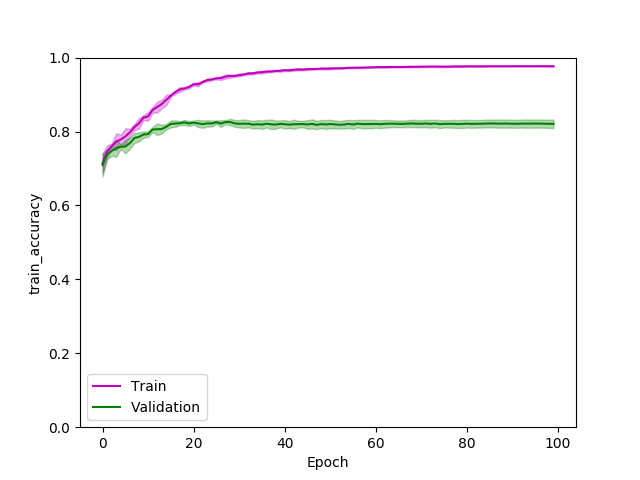
\includegraphics[width=\textwidth]{pics/d4_train_accuracy_mean_train_test.png}
\caption{$D_4$}\label{fig:d4acctraintest}
\end{minipage}
\caption{Train versus test accuracy for the average of cross-validation folds for input variable subsets}\label{fig:traintestacc}
\end{figure}
% ROC Train versus test
%best
\begin{figure}
\centering
\begin{minipage}{.24\textwidth}
  \centering
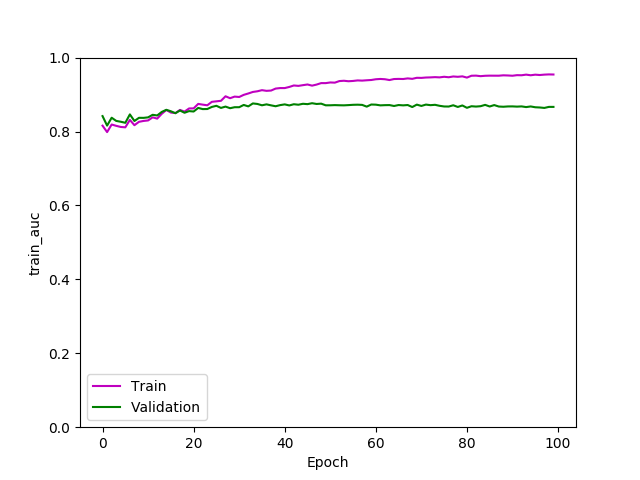
\includegraphics[width=\textwidth]{pics/d1_train_auc_best_train_test.png}
\caption{$D_1$}\label{fig:d1acctraintest}
\end{minipage}
\begin{minipage}{.01\textwidth}
\end{minipage}
\begin{minipage}{.24\textwidth}
  \centering
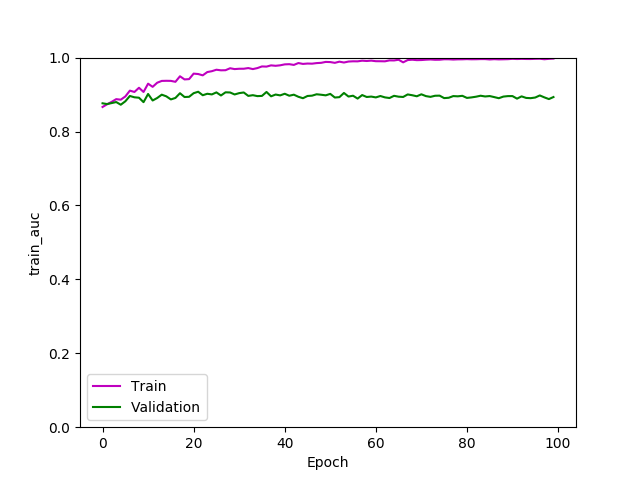
\includegraphics[width=\textwidth]{pics/d2_train_auc_best_train_test.png}
\caption{$D_2$}\label{fig:d2acctraintest}
\end{minipage}
\begin{minipage}{.24\textwidth}
  \centering
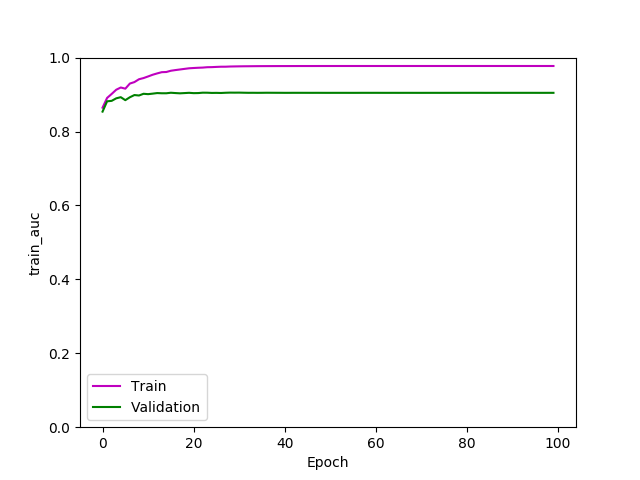
\includegraphics[width=\textwidth]{pics/d3_train_auc_best_train_test.png}
\caption{$D_3$}\label{fig:d3acctraintest}
\end{minipage}
\begin{minipage}{.01\textwidth}
\end{minipage}
\begin{minipage}{.24\textwidth}
  \centering
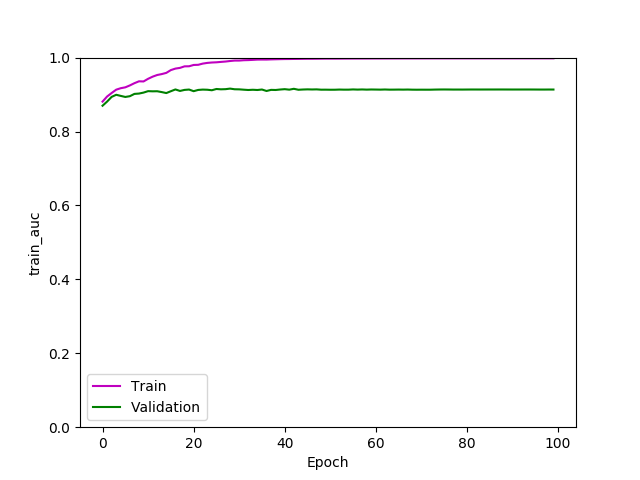
\includegraphics[width=\textwidth]{pics/d4_train_auc_best_train_test.png}
\caption{$D_4$}\label{fig:d4acctraintest}
\end{minipage}
\caption{Train versus test area under the ROC curve for best performing cross-validation fold for input variable subsets}\label{fig:traintestauc}
\end{figure}
%average
\begin{figure}
\centering
\begin{minipage}{.24\textwidth}
  \centering
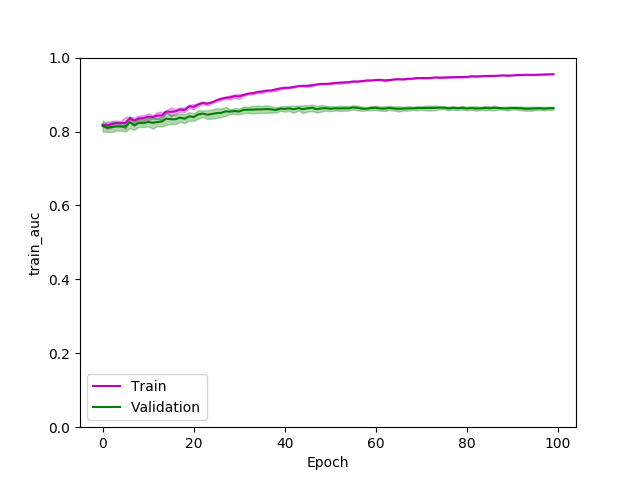
\includegraphics[width=\textwidth]{pics/d1_train_auc_mean_train_test.png}
\caption{$D_1$}\label{fig:d1acctraintest}
\end{minipage}
\begin{minipage}{.01\textwidth}
\end{minipage}
\begin{minipage}{.24\textwidth}
  \centering
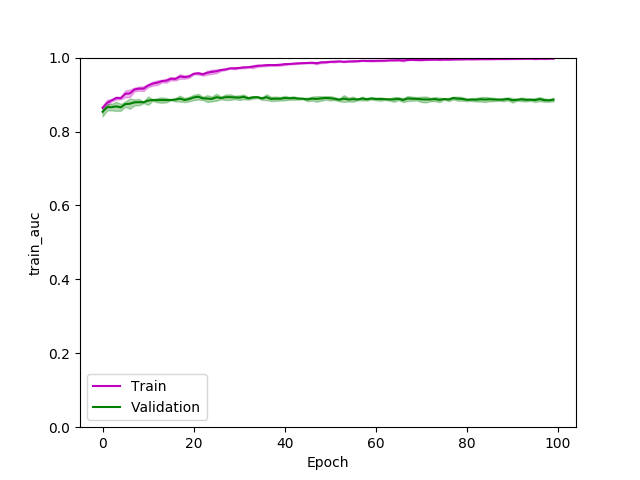
\includegraphics[width=\textwidth]{pics/d2_train_auc_mean_train_test.png}
\caption{$D_2$}\label{fig:d2acctraintest}
\end{minipage}
\begin{minipage}{.24\textwidth}
  \centering
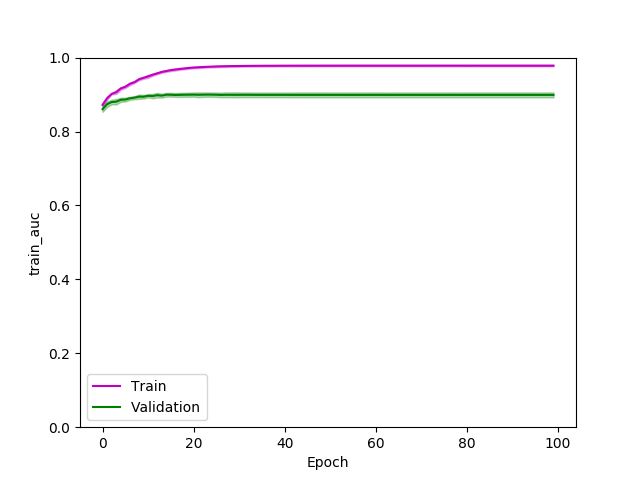
\includegraphics[width=\textwidth]{pics/d3_train_auc_mean_train_test.png}
\caption{$D_3$}\label{fig:d3acctraintest}
\end{minipage}
\begin{minipage}{.01\textwidth}
\end{minipage}
\begin{minipage}{.24\textwidth}
  \centering
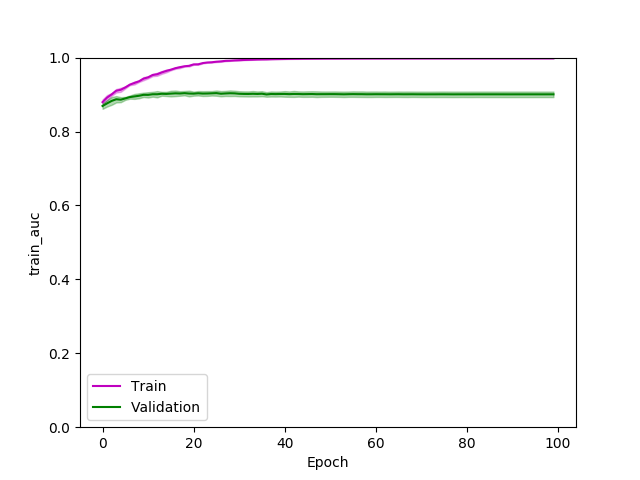
\includegraphics[width=\textwidth]{pics/d4_train_auc_mean_train_test.png}
\caption{$D_4$}\label{fig:d4acctraintest}
\end{minipage}
\caption{Train versus test area under the ROC curve for average of cross-validation folds for input variable subsets}\label{fig:traintestauc}
\end{figure}
% F-measure Train versus test
%best
\begin{figure}
\centering
\begin{minipage}{.24\textwidth}
  \centering
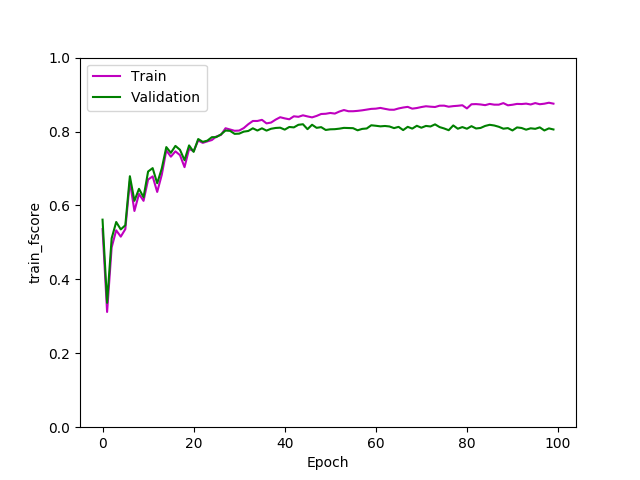
\includegraphics[width=\textwidth]{pics/d1_train_fscore_best_train_test.png}
\caption{$D_1$}\label{fig:d1fscoretraintest}
\end{minipage}
\begin{minipage}{.01\textwidth}
\end{minipage}
\begin{minipage}{.24\textwidth}
  \centering
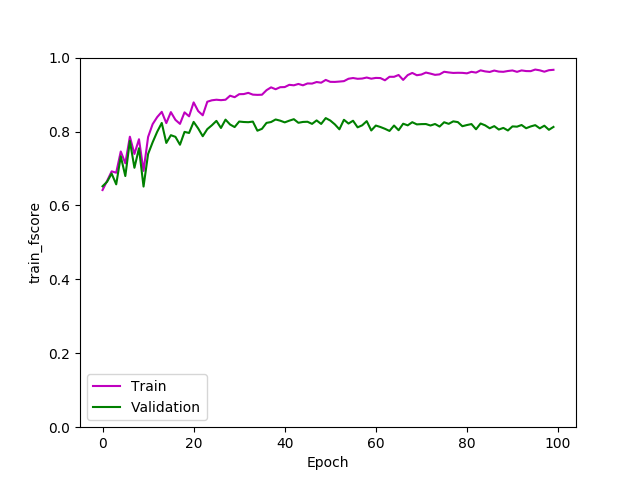
\includegraphics[width=\textwidth]{pics/d2_train_fscore_best_train_test.png}
\caption{$D_2$}\label{fig:d2fscoretraintest}
\end{minipage}
\begin{minipage}{.24\textwidth}
  \centering
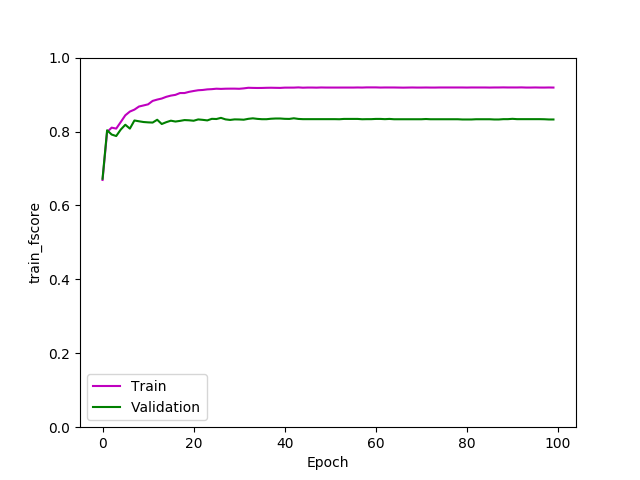
\includegraphics[width=\textwidth]{pics/d3_train_fscore_best_train_test.png}
\caption{$D_3$}\label{fig:d3fscoretraintest}
\end{minipage}
\begin{minipage}{.01\textwidth}
\end{minipage}
\begin{minipage}{.24\textwidth}
  \centering
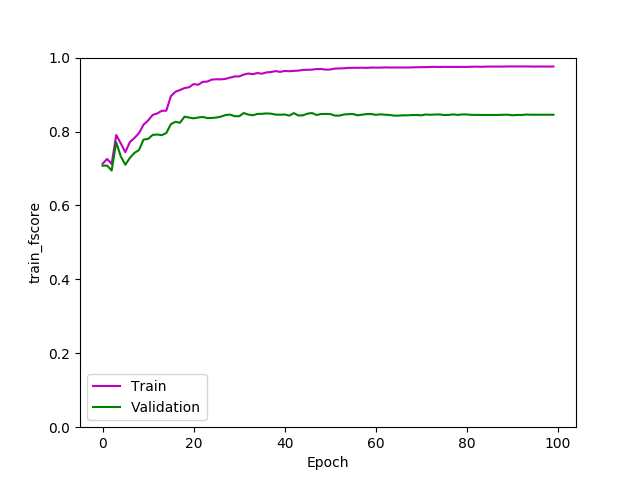
\includegraphics[width=\textwidth]{pics/d4_train_fscore_best_train_test.png}
\caption{$D_4$}\label{fig:d4fscoretraintest}
\end{minipage}
\caption{Train versus test F-score of best performing cross-validation fold for input variable subsets}\label{fig:traintestfscore}
\end{figure}
%average
\begin{figure}
\centering
\begin{minipage}{.24\textwidth}
  \centering
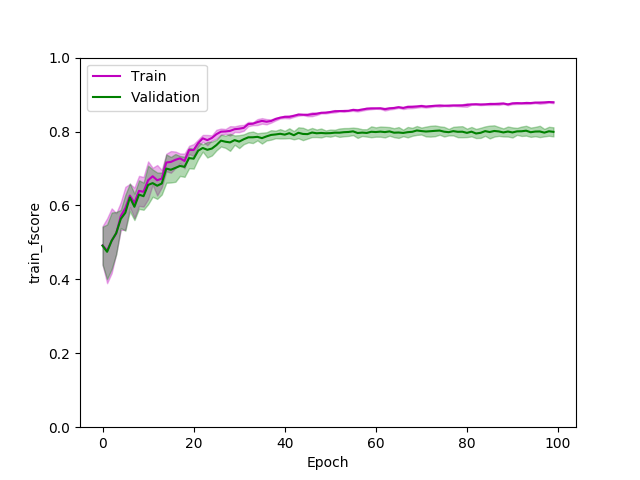
\includegraphics[width=\textwidth]{pics/d1_train_fscore_mean_train_test.png}
\caption{$D_1$}\label{fig:d1fscoretraintest}
\end{minipage}
\begin{minipage}{.01\textwidth}
\end{minipage}
\begin{minipage}{.24\textwidth}
  \centering
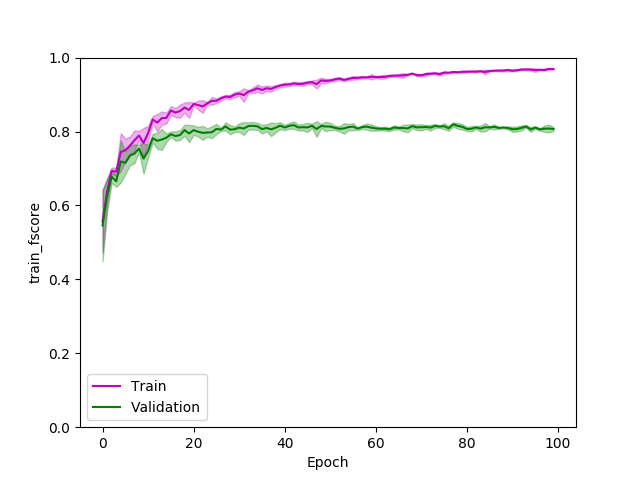
\includegraphics[width=\textwidth]{pics/d2_train_fscore_mean_train_test.png}
\caption{$D_2$}\label{fig:d2fscoretraintest}
\end{minipage}
\begin{minipage}{.24\textwidth}
  \centering
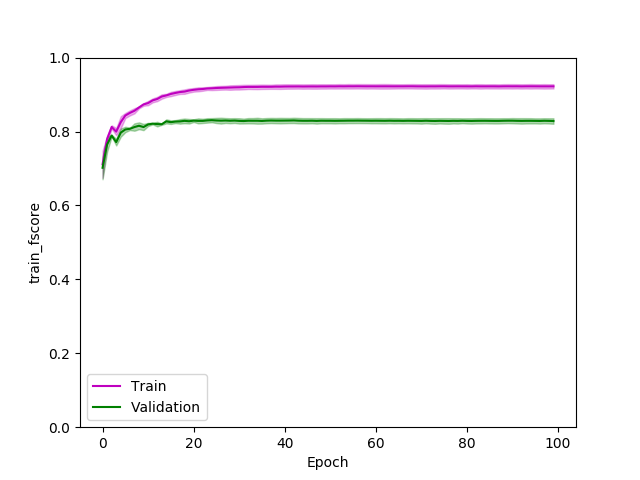
\includegraphics[width=\textwidth]{pics/d3_train_fscore_mean_train_test.png}
\caption{$D_3$}\label{fig:d3fscoretraintest}
\end{minipage}
\begin{minipage}{.01\textwidth}
\end{minipage}
\begin{minipage}{.24\textwidth}
  \centering
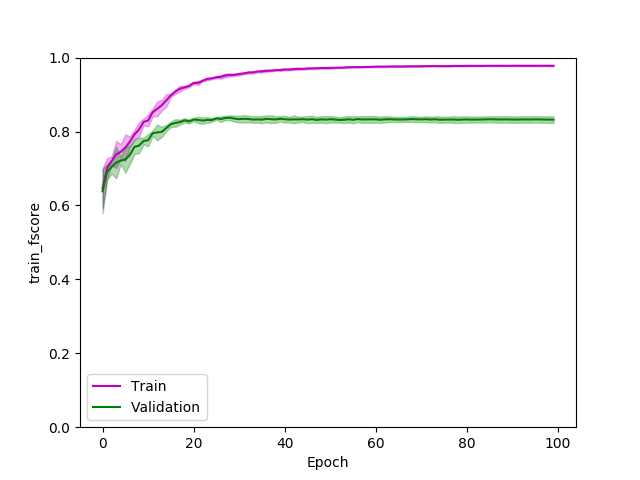
\includegraphics[width=\textwidth]{pics/d4_train_fscore_mean_train_test.png}
\caption{$D_4$}\label{fig:d4fscoretraintest}
\end{minipage}
\caption{Train versus test F-score of average cross-validation score for input variable subsets}\label{fig:traintestfscore}
\end{figure}
% Cross Entropy Train versus test
%best
\begin{figure}
\centering
\begin{minipage}{.24\textwidth}
  \centering
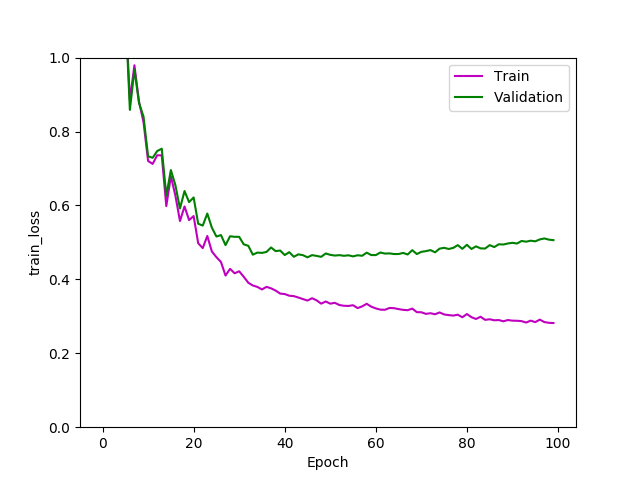
\includegraphics[width=\textwidth]{pics/d1_train_loss_best_train_test.png}
\caption{$D_1$}\label{fig:d1lossraintest}
\end{minipage}
\begin{minipage}{.01\textwidth}
\end{minipage}
\begin{minipage}{.24\textwidth}
  \centering
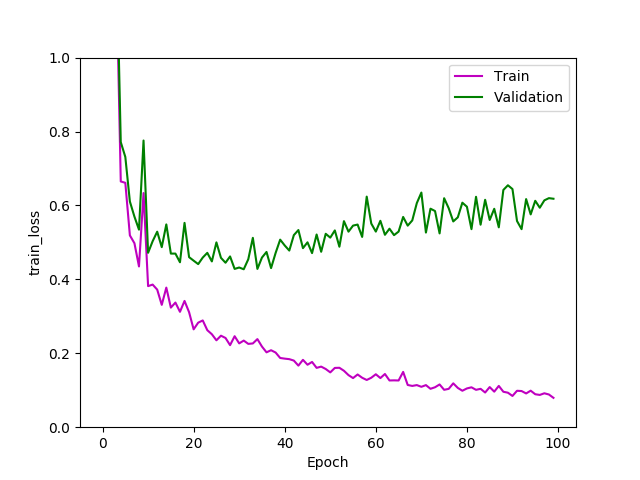
\includegraphics[width=\textwidth]{pics/d2_train_loss_best_train_test.png}
\caption{$D_2$}\label{fig:d2losstraintest}
\end{minipage}
\begin{minipage}{.24\textwidth}
  \centering
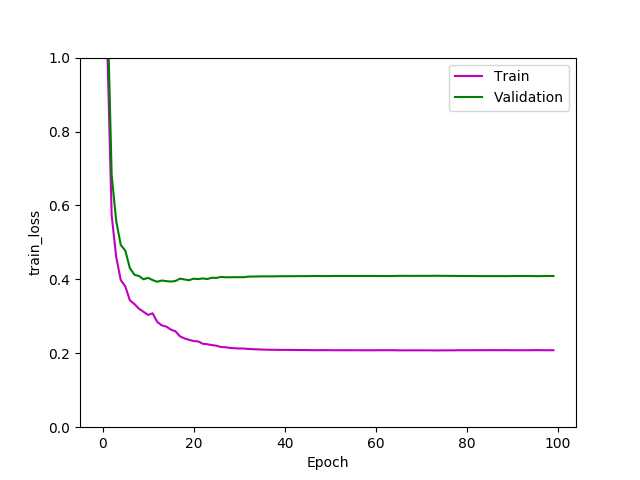
\includegraphics[width=\textwidth]{pics/d3_train_loss_best_train_test.png}
\caption{$D_3$}\label{fig:d3losstraintest}
\end{minipage}
\begin{minipage}{.01\textwidth}
\end{minipage}
\begin{minipage}{.24\textwidth}
  \centering
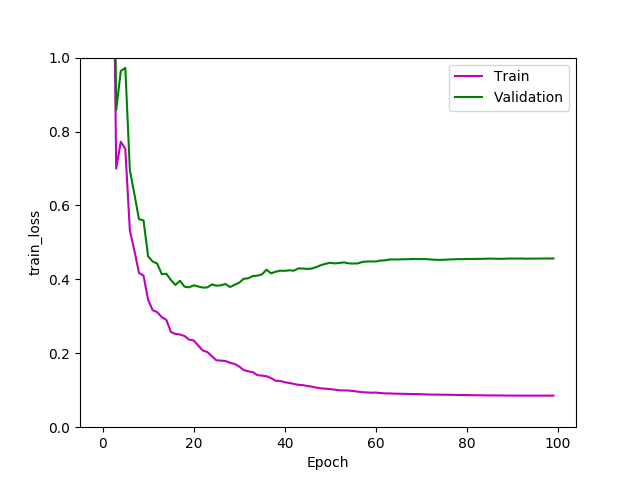
\includegraphics[width=\textwidth]{pics/d4_train_loss_best_train_test.png}
\caption{$D_4$}\label{fig:d4losstraintest}
\end{minipage}
\caption{Train versus test cross entropy loss for best performing cross-validation fold for input variable subsets}\label{fig:traintesloss}
\end{figure}
%average
\begin{figure}
\centering
\begin{minipage}{.24\textwidth}
  \centering
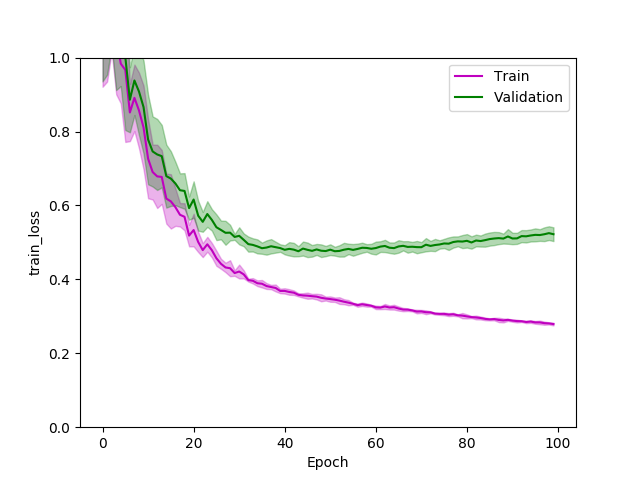
\includegraphics[width=\textwidth]{pics/d1_train_loss_mean_train_test.png}
\caption{$D_1$}\label{fig:d1lossraintest}
\end{minipage}
\begin{minipage}{.01\textwidth}
\end{minipage}
\begin{minipage}{.24\textwidth}
  \centering
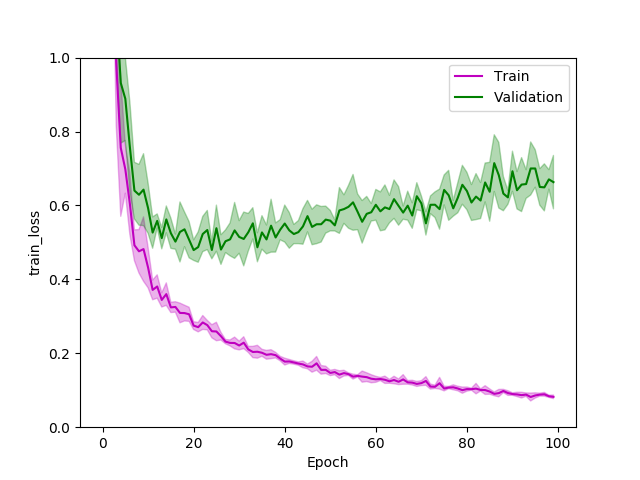
\includegraphics[width=\textwidth]{pics/d2_train_loss_mean_train_test.png}
\caption{$D_2$}\label{fig:d2losstraintest}
\end{minipage}
\begin{minipage}{.24\textwidth}
  \centering
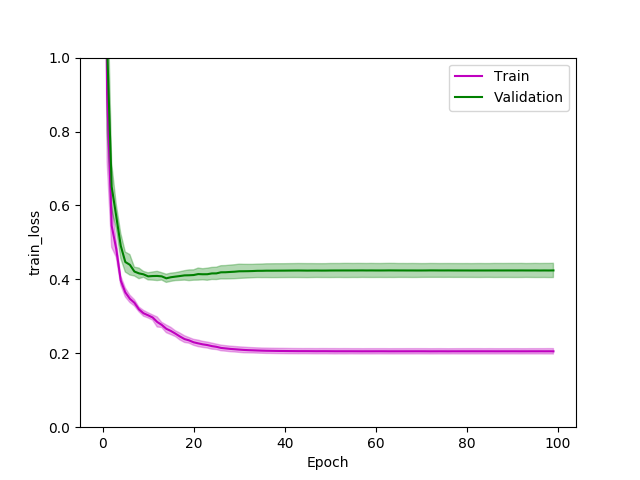
\includegraphics[width=\textwidth]{pics/d3_train_loss_mean_train_test.png}
\caption{$D_3$}\label{fig:d3losstraintest}
\end{minipage}
\begin{minipage}{.01\textwidth}
\end{minipage}
\begin{minipage}{.24\textwidth}
  \centering
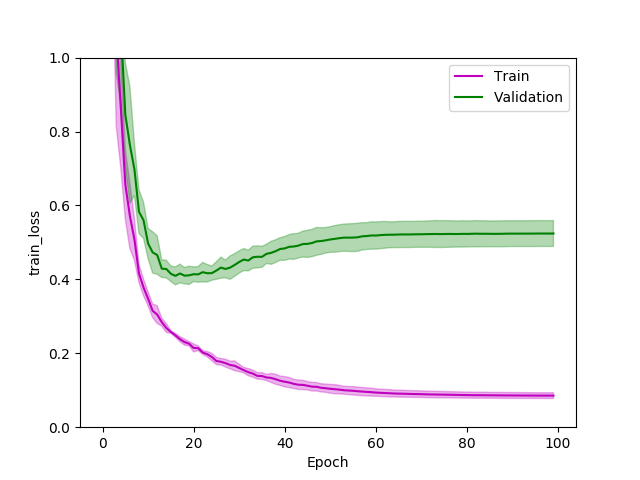
\includegraphics[width=\textwidth]{pics/d4_train_loss_mean_train_test.png}
\caption{$D_4$}\label{fig:d4losstraintest}
\end{minipage}
\caption{Train versus test cross entropy loss for average of cross-validation folds for input variable subsets}\label{fig:traintesloss}
\end{figure}
%================================
% Subsubsection Test performance comparisons across variable partitions
%================================
% Metrics on test
% best
\begin{figure}
\centering
\begin{minipage}{.24\textwidth}
  \centering
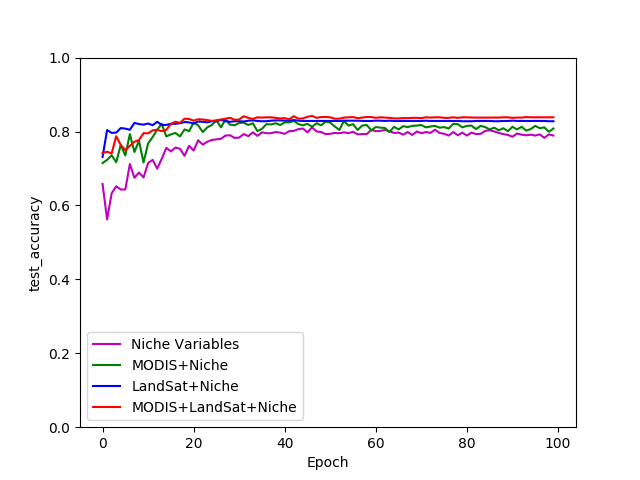
\includegraphics[width=\textwidth]{pics/test_accuracy_variables.png}
\caption{Accuracy}\label{fig:subsetacc}
\end{minipage}
\begin{minipage}{.01\textwidth}
\end{minipage}
\begin{minipage}{.24\textwidth}
  \centering
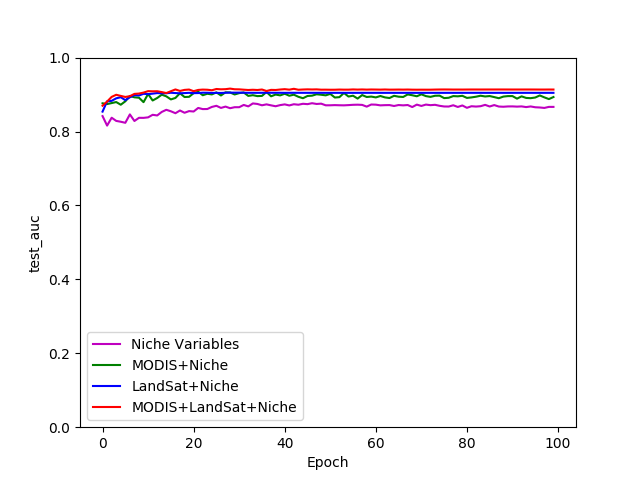
\includegraphics[width=\textwidth]{pics/test_auc_variables.png}
\caption{Area under ROC}\label{fig:subsetauc}
\end{minipage}
\begin{minipage}{.24\textwidth}
  \centering
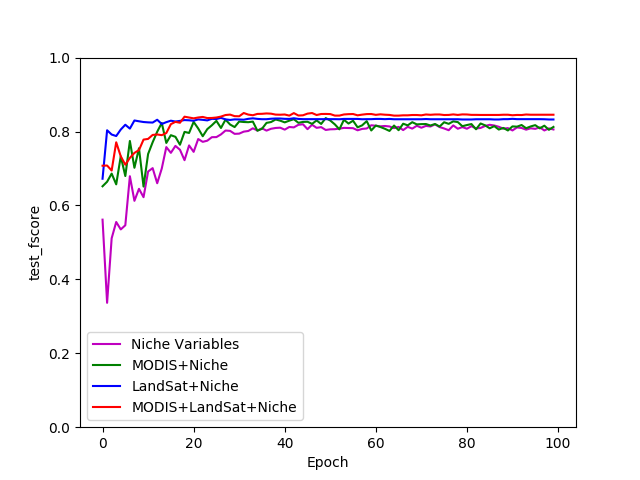
\includegraphics[width=\textwidth]{pics/test_fscore_variables.png}
\caption{F-score}\label{fig:subsetfscore}
\end{minipage}
\begin{minipage}{.01\textwidth}
\end{minipage}
\begin{minipage}{.24\textwidth}
  \centering
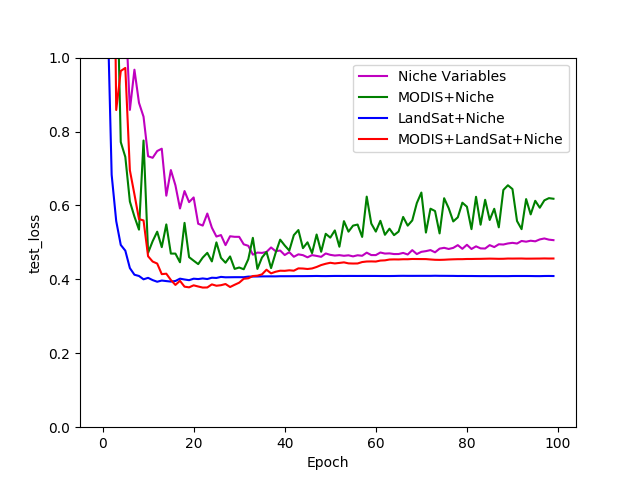
\includegraphics[width=\textwidth]{pics/test_loss_variables.png}
\caption{Cross-entropy}\label{fig:subsetloss}
\end{minipage}
\caption{Test metrics plotted for input variable subsets}\label{fig:testmetrics}
\end{figure}
% average
\begin{figure}
\centering
\begin{minipage}{.24\textwidth}
  \centering
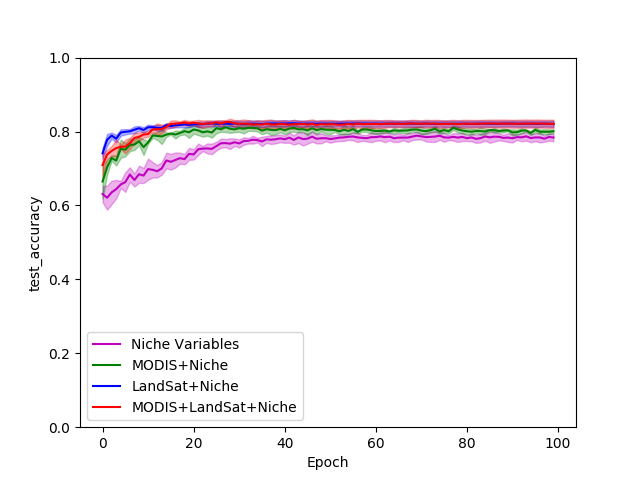
\includegraphics[width=\textwidth]{pics/test_accuracy_mean_variables.png}
\caption{Accuracy}\label{fig:subsetacc}
\end{minipage}
\begin{minipage}{.01\textwidth}
\end{minipage}
\begin{minipage}{.24\textwidth}
  \centering
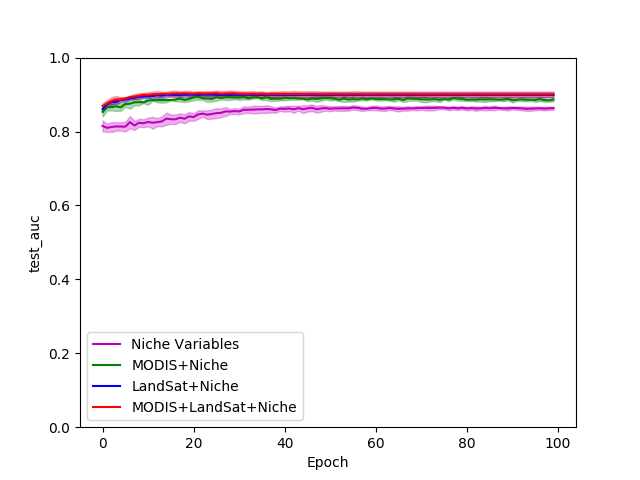
\includegraphics[width=\textwidth]{pics/test_auc_mean_variables.png}
\caption{Area under ROC}\label{fig:subsetauc}
\end{minipage}
\begin{minipage}{.24\textwidth}
  \centering
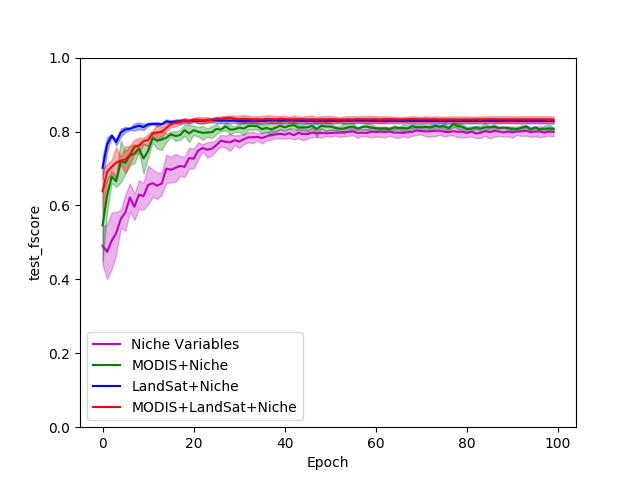
\includegraphics[width=\textwidth]{pics/test_fscore_mean_variables.png}
\caption{F-score}\label{fig:subsetfscore}
\end{minipage}
\begin{minipage}{.01\textwidth}
\end{minipage}
\begin{minipage}{.24\textwidth}
  \centering
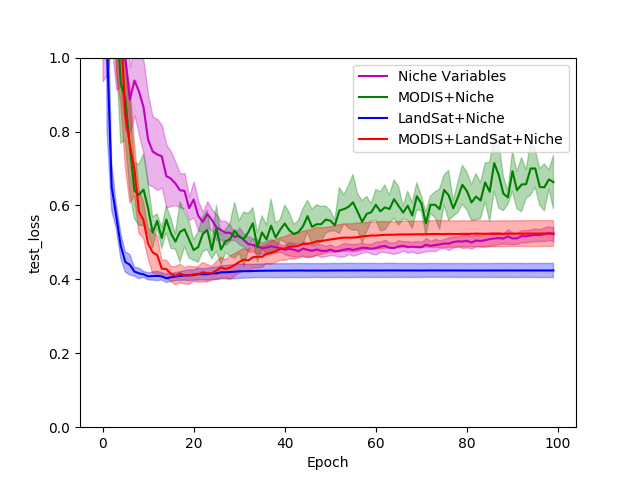
\includegraphics[width=\textwidth]{pics/test_loss_mean_variables.png}
\caption{Cross-entropy}\label{fig:subsetloss}
\end{minipage}
\caption{Test metrics plotted for input variable subsets}\label{fig:testmetrics}
\end{figure}
%================================
% Subsubsection Qualitative assessment
%================================
\subsubsection{Qualitative assesment}
In this section we characterize the overall performance of the best performing DNN models. Figure \ref{confusion} shows a confusion matrix for classification for the best performing DNN model using all the input variables. The types of mistakes the model makes in classification are evenly balanced in terms of false positives and false negatives, however since a smaller proportion of the data contains negative examples it in fact slightly favors false positives. We can see this more clearly in figure 63 which plots accuracy in terms of actual cheat grass coverage values. The worst performance is in the 0-2 percent range which contains only negative examples, so the only mistake that can be made is a false positive. 

Looking closer at prediction performance
we next analyze the model  in terms of accuracy across individual ranges of cheatgrass coverage, ecoregions, land cover classes, and soil and climactic conditions. 
Figures 60-61 show that the models incorporating the LandSat data attain 100 \% accuracy for actual coverage ranging from 70-100 \% cheat grass coverage and accuracy above 90 \% up down to 40 \% coverage. This is despite the fact that there are fewer examples in the data set for these high coverage locations. Since the overwhelming majority of false positives and false negatives fall within the 0-40 \% range, this suggests that changing the class boundary from 2\% to 40\% may lead to more accurate classification at the expense of the overall utility of a final mapping product.
We pay particular interest in judging if the model performs better across different ecoregions due to an unbalanced representation in the data set or something intrinsic in the environment itself.  
Across the other ways of splitting the data into ecoregion, soil moisture temperature regime, and land cover class we see that accuracy is not correlated with frequency of occurrence. Although there does seem to be a minimum threshold for number of examples for an ecoregion to attain acceptable accuracy, considering the low performance of ecoregions 25 and 16 and corresponding small number of examples.  


\begin{itemize}
\item{Map of field data symbolized by classification error}
\end{itemize}
% cheatgrass coverage versus accuracy
% average
\begin{figure}
\centering
\begin{minipage}{.24\textwidth}
  \centering
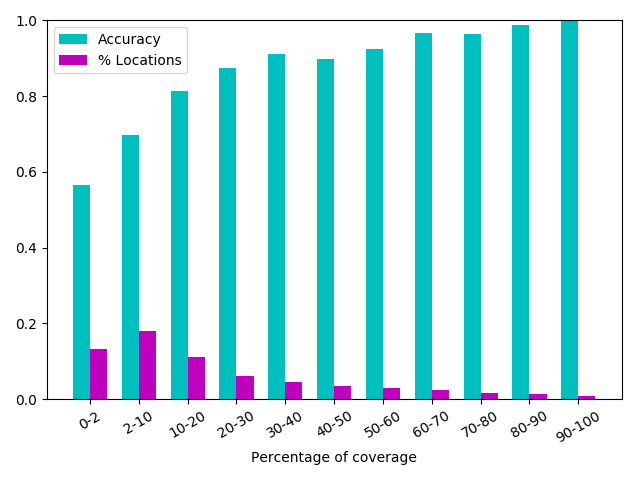
\includegraphics[width=\textwidth]{pics/d1_accuracy_vs_coverage.png}
\caption{$D_1$}
\end{minipage}
\begin{minipage}{.01\textwidth}
\end{minipage}
\begin{minipage}{.24\textwidth}
  \centering
\includegraphics[width=\textwidth]{pics/d2_accuracy_vs_coverage.png}
\caption{$D_2$}
\end{minipage}
\begin{minipage}{.24\textwidth}
  \centering
\includegraphics[width=\textwidth]{pics/d3_accuracy_vs_coverage.png}
\caption{$D_3$}
\end{minipage}
\begin{minipage}{.01\textwidth}
\end{minipage}
\begin{minipage}{.24\textwidth}
  \centering
\includegraphics[width=\textwidth]{pics/d4_accuracy_vs_coverage.png}
\caption{$D_4$}
\end{minipage}
\caption{Accuracy for ranges of cheat grass coverage.}\label{fig:testmetrics}
\end{figure}
% accuracy versus categories
% average
\begin{figure}
\centering
\begin{minipage}{.24\textwidth}
  \centering
\includegraphics[width=\textwidth]{pics/d4_accuracy_vs_coverage.png}
\caption{$D_1$}
\end{minipage}
\begin{minipage}{.01\textwidth}
\end{minipage}
\begin{minipage}{.24\textwidth}
  \centering
\includegraphics[width=\textwidth]{pics/d4_accuracy_vs_ecoregion.png}
\caption{$D_2$}
\end{minipage}
\begin{minipage}{.24\textwidth}
  \centering
\includegraphics[width=\textwidth]{pics/d4_accuracy_vs_landcover.png}
\caption{$D_3$}
\end{minipage}
\begin{minipage}{.01\textwidth}
\end{minipage}
\begin{minipage}{.24\textwidth}
  \centering
\includegraphics[width=\textwidth]{pics/d4_accuracy_vs_soil.png}
\caption{$D_4$}
\end{minipage}
\caption{Accuracy for different subsets of the field locations.}\label{fig:testmetrics}
\end{figure}
% accuracy versus categories
% average
\begin{figure}
\centering
\begin{minipage}{.48\textwidth}
  \centering
\includegraphics[width=\textwidth]{pics/roc.png}
\caption{ROC curves for best performing DNN models on different data subsets}
\end{minipage}
\begin{minipage}{.04\textwidth}
\end{minipage}
\begin{minipage}{.48\textwidth}
  \centering
\includegraphics[width=\textwidth]{pics/confusion_MODIS+LandSat+Niche.png}
\caption{Confusion matrix for best performing DNN model.}\label{confusion}
\end{minipage}
\end{figure}
%============================================================================================
% Subsection Performance on Full Study Region================================================
%=============================================================================================
\subsection{Performance on Full Study Region}
In this section we analyze the geographic variability in cross-validation model predictions among other things.
%\begin{figure}
%\includegraphics[width=\textwidth]{pics/modus_prob.png}
%\caption{250 meter resolution map for best deep neural network classification model.}\label{250m}
%\end{figure}
\subsubsection{Pixel-wise count of cheatgrass class across model predictions}
\subsubsection{Block statistics (count) of cheatgrass class (analogous to block area), then look at range of block counts}
%============================================================================================
%============================================================================================
%Section: Conclusion and Future Work================================================
%=============================================================================================
%============================================================================================
\section{Conclusion and Future Work}
\nocite{*}
\bibliography{fiery}
\bibliographystyle{acm}

\end{document}
































